\documentclass[a4paper,twocolumn,10pt]{ctexart}
% Preamble for the Chinese two-column drafts (自动化学报 / Chinese conference style).
% Requires: \documentclass[twocolumn,10pt]{ctexart} before % Preamble for the Chinese two-column drafts (自动化学报 / Chinese conference style).
% Requires: \documentclass[twocolumn,10pt]{ctexart} before % Preamble for the Chinese two-column drafts (自动化学报 / Chinese conference style).
% Requires: \documentclass[twocolumn,10pt]{ctexart} before \input{preamble}.
\usepackage{amsmath,amssymb,amsthm,mathtools}
\usepackage{graphicx}
\usepackage{booktabs,multirow,array,tabularx}
\usepackage[caption=false]{subfig}
\usepackage{algorithm}
\usepackage{algpseudocode}
\usepackage[margin=2cm]{geometry}
\usepackage{url}
\usepackage{textcomp}
\usepackage{microtype}
\usepackage{xcolor}
\usepackage{bm}
\usepackage[hidelinks]{hyperref}

\setCJKmainfont{Noto Serif CJK SC}
\setCJKsansfont{Noto Sans CJK SC}
\setCJKmonofont{Noto Sans CJK SC}

\graphicspath{{figures/}}
\linespread{1.15}
\raggedbottom
\setlength{\emergencystretch}{2em}
\setlength{\columnsep}{0.75cm}
\renewcommand{\figurename}{图}
\renewcommand{\tablename}{表}
\renewcommand{\refname}{参考文献}
\floatname{algorithm}{算法}
\algrenewcommand\algorithmicrequire{\textbf{输入：}}
\algrenewcommand\algorithmicensure{\textbf{输出：}}

% Independent counters for lemmas / theorems / propositions so that the numbering
% matches the English source (Lemma 1, Theorem 1, Lemmas 2--5, Theorems 2--3,
% Propositions 1--3), see en/preamble.tex.
\newtheorem{theorem}{定理}
\newtheorem{lemma}{引理}
\newtheorem{proposition}{命题}
\newtheorem{corollary}{推论}
\theoremstyle{definition}
\newtheorem{definition}{定义}
\newtheorem{assumption}{假设}
\newtheorem{example}{例}
\theoremstyle{remark}
\newtheorem{remark}[theorem]{注}

\newcommand{\R}{\mathbb{R}}
\newcommand{\Sm}{\mathbb{S}}
\newcommand{\bq}{\mathbf{q}}
\newcommand{\bt}{\mathbf{t}}
\newcommand{\bx}{\mathbf{x}}
\newcommand{\bu}{\mathbf{u}}
\newcommand{\br}{\mathbf{r}}
\newcommand{\bM}{\mathbf{M}}
\newcommand{\bD}{\mathbf{D}}
\newcommand{\bG}{\mathbf{G}}
\newcommand{\bH}{\mathbf{H}}
\newcommand{\bE}{\mathbf{E}}
\newcommand{\bJ}{\mathbf{J}}
\newcommand{\vtwo}{v_2}
\newcommand{\tr}{\operatorname{tr}}
\newcommand{\rank}{\operatorname{rank}}
\newcommand{\diag}{\operatorname{diag}}
\newcommand{\Proj}{\operatorname{Proj}}
\newcommand{\argmin}{\operatorname*{arg\,min}}

\newcommand{\pend}[1]{\textcolor{red}{[#1]}}
\newcommand{\ev}[1]{\emph{#1}}
.
\usepackage{amsmath,amssymb,amsthm,mathtools}
\usepackage{graphicx}
\usepackage{booktabs,multirow,array,tabularx}
\usepackage[caption=false]{subfig}
\usepackage{algorithm}
\usepackage{algpseudocode}
\usepackage[margin=2cm]{geometry}
\usepackage{url}
\usepackage{textcomp}
\usepackage{microtype}
\usepackage{xcolor}
\usepackage{bm}
\usepackage[hidelinks]{hyperref}

\setCJKmainfont{Noto Serif CJK SC}
\setCJKsansfont{Noto Sans CJK SC}
\setCJKmonofont{Noto Sans CJK SC}

\graphicspath{{figures/}}
\linespread{1.15}
\raggedbottom
\setlength{\emergencystretch}{2em}
\setlength{\columnsep}{0.75cm}
\renewcommand{\figurename}{图}
\renewcommand{\tablename}{表}
\renewcommand{\refname}{参考文献}
\floatname{algorithm}{算法}
\algrenewcommand\algorithmicrequire{\textbf{输入：}}
\algrenewcommand\algorithmicensure{\textbf{输出：}}

% Independent counters for lemmas / theorems / propositions so that the numbering
% matches the English source (Lemma 1, Theorem 1, Lemmas 2--5, Theorems 2--3,
% Propositions 1--3), see en/preamble.tex.
\newtheorem{theorem}{定理}
\newtheorem{lemma}{引理}
\newtheorem{proposition}{命题}
\newtheorem{corollary}{推论}
\theoremstyle{definition}
\newtheorem{definition}{定义}
\newtheorem{assumption}{假设}
\newtheorem{example}{例}
\theoremstyle{remark}
\newtheorem{remark}[theorem]{注}

\newcommand{\R}{\mathbb{R}}
\newcommand{\Sm}{\mathbb{S}}
\newcommand{\bq}{\mathbf{q}}
\newcommand{\bt}{\mathbf{t}}
\newcommand{\bx}{\mathbf{x}}
\newcommand{\bu}{\mathbf{u}}
\newcommand{\br}{\mathbf{r}}
\newcommand{\bM}{\mathbf{M}}
\newcommand{\bD}{\mathbf{D}}
\newcommand{\bG}{\mathbf{G}}
\newcommand{\bH}{\mathbf{H}}
\newcommand{\bE}{\mathbf{E}}
\newcommand{\bJ}{\mathbf{J}}
\newcommand{\vtwo}{v_2}
\newcommand{\tr}{\operatorname{tr}}
\newcommand{\rank}{\operatorname{rank}}
\newcommand{\diag}{\operatorname{diag}}
\newcommand{\Proj}{\operatorname{Proj}}
\newcommand{\argmin}{\operatorname*{arg\,min}}

\newcommand{\pend}[1]{\textcolor{red}{[#1]}}
\newcommand{\ev}[1]{\emph{#1}}
.
\usepackage{amsmath,amssymb,amsthm,mathtools}
\usepackage{graphicx}
\usepackage{booktabs,multirow,array,tabularx}
\usepackage[caption=false]{subfig}
\usepackage{algorithm}
\usepackage{algpseudocode}
\usepackage[margin=2cm]{geometry}
\usepackage{url}
\usepackage{textcomp}
\usepackage{microtype}
\usepackage{xcolor}
\usepackage{bm}
\usepackage[hidelinks]{hyperref}

\setCJKmainfont{Noto Serif CJK SC}
\setCJKsansfont{Noto Sans CJK SC}
\setCJKmonofont{Noto Sans CJK SC}

\graphicspath{{figures/}}
\linespread{1.15}
\raggedbottom
\setlength{\emergencystretch}{2em}
\setlength{\columnsep}{0.75cm}
\renewcommand{\figurename}{图}
\renewcommand{\tablename}{表}
\renewcommand{\refname}{参考文献}
\floatname{algorithm}{算法}
\algrenewcommand\algorithmicrequire{\textbf{输入：}}
\algrenewcommand\algorithmicensure{\textbf{输出：}}

% Independent counters for lemmas / theorems / propositions so that the numbering
% matches the English source (Lemma 1, Theorem 1, Lemmas 2--5, Theorems 2--3,
% Propositions 1--3), see en/preamble.tex.
\newtheorem{theorem}{定理}
\newtheorem{lemma}{引理}
\newtheorem{proposition}{命题}
\newtheorem{corollary}{推论}
\theoremstyle{definition}
\newtheorem{definition}{定义}
\newtheorem{assumption}{假设}
\newtheorem{example}{例}
\theoremstyle{remark}
\newtheorem{remark}[theorem]{注}

\newcommand{\R}{\mathbb{R}}
\newcommand{\Sm}{\mathbb{S}}
\newcommand{\bq}{\mathbf{q}}
\newcommand{\bt}{\mathbf{t}}
\newcommand{\bx}{\mathbf{x}}
\newcommand{\bu}{\mathbf{u}}
\newcommand{\br}{\mathbf{r}}
\newcommand{\bM}{\mathbf{M}}
\newcommand{\bD}{\mathbf{D}}
\newcommand{\bG}{\mathbf{G}}
\newcommand{\bH}{\mathbf{H}}
\newcommand{\bE}{\mathbf{E}}
\newcommand{\bJ}{\mathbf{J}}
\newcommand{\vtwo}{v_2}
\newcommand{\tr}{\operatorname{tr}}
\newcommand{\rank}{\operatorname{rank}}
\newcommand{\diag}{\operatorname{diag}}
\newcommand{\Proj}{\operatorname{Proj}}
\newcommand{\argmin}{\operatorname*{arg\,min}}

\newcommand{\pend}[1]{\textcolor{red}{[#1]}}
\newcommand{\ev}[1]{\emph{#1}}

\begin{document}
\pagestyle{plain}
\zihao{5}

\title{\zihao{2}\bfseries Robust-QPEPLayer：面向无RANSAC鲁棒位姿估计的曲率修正隐式微分}
\author{\zihao{4} 第一作者\quad 第二作者\\[2pt] \zihao{5}（[单位名称]，[城市] [邮编]）}
\date{}
\maketitle

\begin{abstract}
\zihao{-5}
可微位姿估计层使端到端学习能够穿过几何优化，但现有方法在粗大外点下容易失效：它们要么在可认证求解器外再包一层不可微的RANSAC前端，要么以冻结或沿迭代展开的权重微分局部鲁棒$M$估计器。本文提出\textbf{Robust-QPEPLayer}，一种无RANSAC的可微位姿层，融合Black--Rangarajan（BR）对偶、渐进非凸（GNC）与恒定规模的四元数位姿求解器（QPEP）。前向交替执行闭式外点权重更新与全局求解的加权QPEP，对应数量仅通过$O(N)$累加进入；反向以$6\times6$系统精确微分鲁棒不动点，并对GNC迭代次数保持$O(1)$内存，其中包含重降曲率修正与单位四元数乘子项。我们证明Geman--McClure核的精确BR对偶、曲率修正的Schur补恒等式，以及$\mathbb{S}^3\times\mathbb{R}^3$上的精确黎曼Hessian；一维命题表明冻结权重微分会翻转导数符号，逐观测$O(\|\mathbf{r}_i\|^{-4})$界把梯度衰减与前向鲁棒性区分开。精确Jacobian与中心差分吻合到$3$--$5\times10^{-8}$，而冻结权重的边界相对误差为$1.07$、余弦为$0.234$。GNC-GM在$70\%$随机外点以内与固定1000次RANSAC成功率相当，运行时间低$22$--$32\times$；在全部八个官方3DMatch测试场景、全部11个KITTI odometry序列00--10以及四次UTIAS In-The-Dark运行上，误差为$0.078$--$0.150^\circ$与$0.007$--$0.020$~m。

\end{abstract}

\noindent{\zihao{-5}\textbf{关键词：}鲁棒位姿估计；可微优化；Black--Rangarajan对偶；渐进非凸；隐式微分}

\noindent{\zihao{-5}\textbf{中图分类号：}TP242\quad\textbf{文献标志码：}A}

\section{引言}

优化层已成为可微机器人与视觉中的标准构件：在前向中求解一个几何问题，再对其最优性条件做隐式微分，从而为上游网络提供梯度\cite{holmes2025sdpr,pineda2022theseus,chen2020bpn}。对位姿估计而言，困难在于非凸性：局部求解器收敛到\emph{某个}驻点，其梯度一般并不是全局位姿的梯度。SDPRLayers \cite{holmes2025sdpr}求解一个凸半定松弛，认证秩一最优性，并在该处对原始KKT系统求微分；QPEP \cite{wu2022qpep}消去平移，用Gr\"obner基枚举一个四次系统的全部驻点，返回代数意义下的全局最优解。二者前向都是全局的，但都不鲁棒：SDPRLayers的真实数据实验把该层包在RANSAC \cite{fischler1981ransac}中并在干净样本上训练，而带逐对应二值变量的鲁棒SDP会把$10\times10$矩阵提升为$(10+9N)\times(10+9N)$ \cite{holmes2025sdpr}。

本文提出的问题是：\emph{能否得到一个可微位姿层，它对粗大外点鲁棒、维数关于对应数量恒定，并且精确微分鲁棒估计器，而不是展开迭代或冻结其权重？}我们以三个要素作答：\textbf{Black--Rangarajan对偶} \cite{black1996br}，它把重降$M$估计器转化为关于位姿与每个对应一个权重的联合优化；\textbf{渐进非凸} \cite{yang2020gnc,yang2020teaser}，它把凸代理逐步退火到重降核；以及\textbf{QPEP} \cite{wu2022qpep}，它在固定个数的变量中全局求解每个加权子问题。三者的组合在思想上并不新颖——以加权最小二乘为内层求解器的GNC在鲁棒配准中已是标准做法 \cite{yang2020gnc,yang2020teaser}——但\emph{可微}层暴露出一种据我们所知尚未被单独隔离的结构：鲁棒不动点的精确导数包含一个\emph{重降曲率修正}，它正是BR权重块的Schur补；在$\mathbb{S}^3$上它还包含一个\emph{约束乘子项}，这是欧氏公式所遗漏的。丢掉其中任何一项都会使梯度产生数量级错误，甚至对边界外点翻转其符号。

\subsection{贡献}

\begin{enumerate}
\item \textbf{恒定维数的鲁棒前向过程与精确对偶。}Geman--McClure（GM）核的BR对偶对任意权重与退火参数都精确成立，最优权重即核的导数，GNC-QPEP是单调块坐标下降，其极限点是逐坐标驻点（引理~\ref{lem:brdual}、定理~\ref{thm:gnc}）。内层加权子问题被全局求解；在3D--3D实验中它化为闭式$4\times4$特化。
\item \textbf{带曲率修正的精确不动点隐式微分。}GNC不动点是鲁棒代价的驻点（引理~\ref{lem:fixedpoint}）；重降修正就是被消去的权重块（引理~\ref{lem:schur}）；精确黎曼Hessian包含$-\lambda_{\mathrm{rob}}\diag(I_3,0_3)$，其中3D--3D常数为$\lambda_i=4\mathbf{u}_i^\top W_i\mathbf{r}_i$，\emph{不是}$4e_i$（引理~\ref{lem:hessian}）。丢掉它会使谱改变$O(1)$。
\item \textbf{严格的符号翻转结果与$O(\|\mathbf{r}\|^{-4})$梯度界。}在一维位置模型中，于$H_{\mathrm{rob}}>0$的严格极小点处，精确导数为$\lambda_\parallel(e_j)/H_{\mathrm{rob}}$，而冻结权重导数恒为正；当$e_j>c^2/3$时二者符号严格相反（命题~\ref{prop:signflip}），且对两个充分分离的观测此构型确实存在（命题~\ref{prop:existence}）。我们还证明，在一致可逆性下逐观测有$\|\partial z^*/\partial\mathbf{y}_i\|=O(\|\mathbf{r}_i\|^{-4})$界，而前向偏差仅为$O(\|\mathbf{r}_i\|^{-3})$（命题~\ref{prop:bound}）。
\item \textbf{统一的核框架与评测协议。}我们给出GM、Cauchy、Welsch与TLS的BR对偶，其前向与反向在结构上完全相同（附录~\ref{app:kernel}），并在合成3D--3D、ModelNet40/10、全部八个官方3DMatch测试场景、两次KITTI raw驾驶、全部11个KITTI odometry序列00--10（每个33个选定帧）以及四次UTIAS In-The-Dark运行上进行评测。Theseus与SDPRLayers作为外部基线。
\end{enumerate}

该层与Veronese提升及受约束QPEP形式互补：它既不使用$O(10)$的Veronese同构，也不使用不等式约束，只共用QPEP内层求解器。

\section{相关工作}
\label{sec:related}

\noindent\textbf{可认证与全局位姿层。}SDPRLayers \cite{holmes2025sdpr}把一个齐次QCQP提升为Shor半定规划，认证秩一最优性，并用隐式选择论证对原始KKT系统求微分。其保证以紧性为条件；其真实数据流程使用RANSAC与干净样本，且其半定规划随变量数增长。QPEP \cite{wu2022qpep}消去平移，用Gr\"obner基求解一个四次系统，返回带协方差的代数全局位姿，但没有梯度层。我们把QPEP的标量权重$4\times4$特化用作\emph{子程序}，并添加鲁棒外循环与精确反向；我们不声称鲁棒代价的可认证全局最优性。

\noindent\textbf{局部可微优化。}Theseus \cite{pineda2022theseus}在Lie群上提供可微非线性最小二乘，支持隐式微分与直接损失最小化。它把鲁棒核作为软代价加以支持，但其不动点是惩罚目标的局部驻点，不暴露重降曲率修正，且核是作为标量权重施加，而非通过BR对偶。BPnP \cite{chen2020bpn}通过隐函数定理穿过PnP求解器反传，没有外点机制。EPro-PnP \cite{chen2022epropnp}用Boltzmann分布建模位姿歧义；它互补但方差大，且不是重降$M$估计器。Pyatov等 \cite{pyatov2024robust}把鲁棒两视图几何视为带可学习匹配置信权重的隐式层，属2D--2D范围；我们的是$\mathbb{S}^3\times\mathbb{R}^3$上的度量3D--3D位姿，并有显式二阶理论。POLI \cite{poli2026}学习逐点高斯几何，可提供各向异性$W_i$；它是前端表示而非鲁棒位姿层，而我们的$W_i$可以是POLI的椭球。

\noindent\textbf{鲁棒估计与隐式层。}BR对偶 \cite{black1996br}统一了外点过程与鲁棒统计，并给出我们所使用的对偶形式。GNC由Yang等 \cite{yang2020gnc}与TEASER \cite{yang2020teaser}在空间感知中推广，后者把GNC-TLS与可认证的旋转子问题结合；我们的内层问题是完整的6-DoF QPEP，贡献在于\emph{可微}不动点。GM、Cauchy、Welsch与TLS核都是经典核 \cite{geman1985}，其BR对偶见附录~C。RANSAC \cite{fischler1981ransac}是不可微的替代方案，比较时始终注明其预算。无Jacobian反传 \cite{fung2022jfb}用廉价近似替代逆Jacobian求解；冻结鲁棒权重是一种类似的“幻影梯度”，但我们的一维命题表明它可能符号错误。黎曼Hessian公式是嵌入流形的标准公式 \cite{absil2008}。最接近的可微鲁棒层是Pyatov等，最接近的鲁棒全局求解器是TEASER/GNC，最接近的位姿层是SDPRLayers；我们的区别点在于带曲率修正的精确鲁棒不动点微分、黎曼约束项、一维符号翻转定理、$O(\|\mathbf{r}\|^{-4})$界，以及恒定维数的QPEP内层求解器。

\section{问题建模与符号}
\label{sec:formulation}

令$\mathcal{M}=\mathbb{S}^3\times\mathbb{R}^3$，$z=(\mathbf{q},\mathbf{t})$且$\mathbf{q}^\top\mathbf{q}=1$。对$i=1,\dots,N$，令$\mathbf{p}_i\in\mathbb{R}^3$为模型点，$\mathbf{y}_i\in\mathbb{R}^3$为观测，$W_i\in\mathbb{S}^3_{++}$为正定权重。3D--3D残差及其平方加权范数为
\begin{equation}
\begin{aligned}
\mathbf{r}_i(z,\theta)&=R(\mathbf{q})\mathbf{p}_i+\mathbf{t}-\mathbf{y}_i,\\
e_i(z,\theta)&=\|\mathbf{r}_i\|_{W_i}^2=\mathbf{r}_i^\top W_i\mathbf{r}_i\ge0,
\end{aligned}
\end{equation}
其中$\theta$汇集该层的参数（对应、特征，以及可选的权重）。记$\mathbf{u}_i=R(\mathbf{q})\mathbf{p}_i$，$J_i=\partial\mathbf{u}_i/\partial\mathbf{q}\in\mathbb{R}^{3\times4}$；由于$\mathbf{u}_i$关于$\mathbf{q}$是二次齐次的，Euler定理给出$J_i\mathbf{q}=2\mathbf{u}_i$。

鲁棒代价为$F_{\mathrm{rob}}(z;\theta)=\sum_{i=1}^N\rho(e_i(z;\theta))$，其中Geman--McClure核为
\begin{equation}
\begin{aligned}
\rho(e)&=\frac{c^2e}{c^2+e},\qquad
\rho'(e)=\frac{c^4}{(c^2+e)^2},\\
\rho''(e)&=-\frac{2c^4}{(c^2+e)^3}.
\end{aligned}
\end{equation}
GNC代理为$\rho_\mu(e)=\mu c^2e/(\mu c^2+e)$，$\mu\ge1$。BR对偶变量为$w_i\in[0,1]$，对偶势为$\psi_\mu(w)=\mu c^2(\sqrt{w}-1)^2$。记$g_i$与$H_i$为$e_i$在$\mathcal{M}$上的黎曼梯度与Hessian \cite{absil2008}，$g_i^E,H_i^E$为它们在$\mathbb{R}^7$中的欧氏对应量。$P=I_4-\mathbf{q}\mathbf{q}^\top$为$\mathbf{q}$处的切投影；$\Pi=\diag(P,I_3)$；$B=\diag(B_q,I_3)$为正交切基，其中$B_q\in\mathbb{R}^{4\times3}$张成$\{\mathbf{q}\}^{\perp}$。驻点映射为
\begin{equation}
\Phi(z,\theta)=\sum_i\rho'(e_i(z,\theta))\,g_i(z,\theta)\in T_z\mathcal{M}.
\label{eq:phi}
\end{equation}
在$\mu=1$处的GNC不动点满足$w_i=\rho'(e_i)$且$\Phi=0$；精确导数由$H_{\mathrm{rob}}\,\mathrm{d}z+\partial_\theta\Phi\,\mathrm{d}\theta=0$得到。

\noindent\textbf{假设。}(A1) $e_i\in C^2$且所有导数连续；$W_i$位于$\mathbb{S}^3_{++}$的紧子集中。(A2) 加权QPEP由枚举全部KKT根的代数求解器全局求解——这是代数全局假设，不是凸认证。(A3) 在关注点处加权极小点唯一且$H_{\mathrm{rob}}$可逆；对严格局部极小点我们将其加强为$H_{\mathrm{rob}}\succ0$。(A4) 参数光滑地进入；主要推导假设$W_i$固定，$W_i(\theta)$的扩展见附录~\ref{app:proofs}。(A5) $N\ge3$，$\sum_iw_iW_i\succ0$，且3D点不共线。

\section{方法与理论}
\label{sec:method}

\subsection{Black--Rangarajan对偶与GNC-QPEP前向}

\begin{lemma}[GM的精确BR对偶]\label{lem:brdual}
对任意$\mu\ge1$、$c>0$与$e\ge0$，
\begin{equation}
\begin{aligned}
\rho_\mu(e)&=\min_{w\in[0,1]}\big\{we+\psi_\mu(w)\big\},\\
w^*(e)&=\rho_\mu'(e)=\Big(\frac{\mu c^2}{\mu c^2+e}\Big)^2,
\end{aligned}
\end{equation}
从而对任意$z$有
$\min_{w\in[0,1]^N}\sum_i\{w_ie_i(z)+\psi_\mu(w_i)\}=\sum_i\rho_\mu(e_i(z))$。
标量目标在$(0,1]$上严格凸、驻点为$w^*$，盒约束是笛卡尔积；完整证明见附录~\ref{app:proofs}。
\end{lemma}

\begin{theorem}[GNC-QPEP前向]\label{thm:gnc}
在(A1)、(A2)、(A5)下，固定$\mu\ge1$并交替执行
\begin{equation}
\begin{aligned}
w_i^{(k)}&=\rho_\mu'\big(e_i(z^{(k)})\big),\\
z^{(k+1)}&=\argmin_{z\in\mathcal{M}}\sum_iw_i^{(k)}e_i(z).
\end{aligned}
\end{equation}
则：
\begin{enumerate}
\item[(i)] $w$步是精确的，$z$步是加权QPEP。消去$\mathbf{t}$得
  $\mathbf{t}(w,\mathbf{q})=G(w)^{-1}\sum_iw_iW_i(\mathbf{y}_i-R(\mathbf{q})\mathbf{p}_i)$，其中
  $G(w)=\sum_iw_iW_i$；约化代价是关于$\mathbf{q}$的四次多项式，KKT系统有四个（或七个）变量，
  $N$仅通过$O(N)$累加进入固定规模的矩阵。
\item[(ii)] $F_\mu(z^{(k)})$非增；若每个加权极小点唯一，则迭代收敛到不动点
  $(z_\mu^*,w_\mu^*)$，其中$w_{\mu,i}^*=\rho_\mu'(e_i(z_\mu^*))$且
  $z_\mu^*\in\argmin_z\sum_iw_{\mu,i}^*e_i(z)$。
\item[(iii)] 当$\mu\downarrow1$时，每个聚点满足$w_i^*=\rho'(e_i(z^*))$且
  $\Phi(z^*)=0$，即$z^*$是$F_{\mathrm{rob}}$的驻点。
\item[(iv)] 全局性质只属于内层加权QPEP：外层GNC是非凸块坐标方法，可能停在鞍点；相干多数外点
  还可使$F_{\mathrm{rob}}$的全局极小点本身出错（第~\ref{sec:discussion}节）。
\end{enumerate}
陈述(ii)是标准的单调块下降论证；(iii)由$\rho_\mu'$的连续性与加权问题的一阶条件得到。在
3D--3D实验中，内层求解器是QPEP的闭式标量权重$4\times4$特化；$4\times4$的Davenport/Horn
变体在附录~\ref{app:systems}中做了基准测试。
\end{theorem}

\begin{algorithm}[t]
\caption{前向GNC-QPEP（一次鲁棒求解）}
\label{alg:forward}
\footnotesize
\begin{algorithmic}[1]
\Require $\{(\mathbf{p}_i,\mathbf{y}_i,W_i)\}_{i=1}^N$，尺度$c$，调度$\gamma$
\State 初始化$\mathbf{q},\mathbf{t}$；$\mu\gets3\max_ie_i/c^2$
\While{$\mu\ge1$}
  \For{$k=1$ to $K$}
    \State 对所有$i$：$e_i\gets\|R(\mathbf{q})\mathbf{p}_i+\mathbf{t}-\mathbf{y}_i\|_{W_i}^2$
    \State 对所有$i$：$w_i\gets\big(\mu c^2/(\mu c^2+e_i)\big)^2$
    \State $(\mathbf{q},\mathbf{t})\gets\textsc{QPEP-Global}\big(\sum_iw_ie_i\big)$
  \EndFor
  \State $\mu\gets\max(1,\mu/\gamma)$
\EndWhile
\State \Return $\mathbf{q},\mathbf{t},w,e$
\end{algorithmic}
\end{algorithm}

退火调度为$\mu_0\ge3\max_ie_i(z^{(0)})/c^2$，$\mu_{k+1}=\max(1,\mu_k/\gamma)$，
$\gamma\in[1.2,2.0]$，内层交替次数固定或自适应。$\mu_0$的选取使每个残差的\emph{径向}二阶导数
为正；它并不使完整代价关于$z$凸。

\subsection{不动点、曲率修正与精确黎曼Hessian}

\begin{lemma}[不动点$\Rightarrow$驻性]\label{lem:fixedpoint}
若$z^*$全局极小化$\sum_iw_i^*e_i$且$w_i^*=\rho'(e_i(z^*))$，则$(z^*,w^*)$是GNC不动点且
$\Phi(z^*)=0$。反之，$\Phi(z^*)=0$加上同样的加权全局极小性质给出不动点；仅有驻性不够。
\end{lemma}

\begin{lemma}[曲率修正$=$Schur补]\label{lem:schur}
在GNC不动点处，令$H_{\mathrm{IRLS}}=\sum_i\rho'(e_i^*)H_i$，
$\Delta H_{\mathrm{redesc}}=\sum_i\rho''(e_i^*)\,g_ig_i^\top\preceq0$，$D=[g_1,\dots,g_N]$，
$\Psi''=\diag(\psi''(w_i^*))$。联合BR目标的Hessian为
\begin{equation}
\begin{aligned}
H_J&=\begin{bmatrix}H_{\mathrm{IRLS}}&D\\D^\top&\Psi''\end{bmatrix},\\
H_{\mathrm{rob}}&=H_{\mathrm{IRLS}}-D\Psi''^{-1}D^\top
=H_{\mathrm{IRLS}}+\Delta H_{\mathrm{redesc}}.
\end{aligned}
\end{equation}
由于$\psi''(w_i^*)=-1/\rho''(e_i^*)>0$，重降修正正是被消去的权重块；且若
$H_{\mathrm{IRLS}}\succeq0$，则$H_J\succ0\iff H_{\mathrm{rob}}\succ0$。冻结权重会删除该
Schur补；第~\ref{sec:gradient}节量化由此产生的梯度误差。
\end{lemma}

\begin{lemma}[$\mathbb{S}^3\times\mathbb{R}^3$上的精确黎曼Hessian]\label{lem:hessian}
令$f\in C^2(\mathcal{M})$，欧氏梯度为$G$、Hessian为$H_E$。则
$\operatorname{Hess}f=\Pi\big(H_E-(\mathbf{q}^\top G_q)\diag(I_4,0_3)\big)\Pi$，且在正交切基$B$下
\begin{equation}
H_f=B^\top H_E B-(\mathbf{q}^\top G_q)\diag(I_3,0_3).
\end{equation}
对$F_{\mathrm{rob}}$，
\begin{equation}
\boxed{
\begin{aligned}
H_{\mathrm{rob}}&=B^\top\Big[\sum_i\rho'(e_i)H_i^E\Big]B\\
&\quad+B^\top\Big[\sum_i\rho''(e_i)g_i^E(g_i^E)^\top\Big]B\\
&\quad-\lambda_{\mathrm{rob}}\diag(I_3,0_3),\\
\lambda_{\mathrm{rob}}&=\mathbf{q}^\top G_q=\sum_i\rho'(e_i)\lambda_i .
\end{aligned}}
\end{equation}
若$H_i$与$g_i$表示黎曼量，则等价形式为
$H_{\mathrm{rob}}=\sum_i\rho'(e_i)H_i+\sum_i\rho''(e_i)g_ig_i^\top$。项
$-\lambda_{\mathrm{rob}}\diag(I_3,0_3)$是单位四元数约束的乘子，不能通过重缩放吸收：对3D--3D，
\begin{equation}
\begin{aligned}
\lambda_i&=\mathbf{q}^\top g_{i,q}^E=4\mathbf{u}_i^\top W_i\mathbf{r}_i\\
&=4\big(e_i-(\mathbf{t}-\mathbf{y}_i)^\top W_i\mathbf{r}_i\big)\neq4e_i
\end{aligned}
\end{equation}
只要$(\mathbf{t}-\mathbf{y}_i)^\top W_i\mathbf{r}_i\neq0$。在球面上，
$f(\mathbf{q})=\frac12\|\mathbf{q}\|^2$为常数、黎曼Hessian为零，而欧氏公式在切坐标下给出
$I_3$。在$c=1.0$的六维3D--3D例子中，未修正公式与测地有限差分Hessian的相对Frobenius范数差为
$25.9\%$，修正后公式吻合到$9.9\times10^{-8}$；乘子为$\lambda_{\mathrm{rob}}=1.033$。
\end{lemma}

\begin{lemma}[3D--3D权重]\label{lem:weights}
沿用上述记号，$g_{i,q}^E=2J_i^\top W_i\mathbf{r}_i$，$g_{i,t}^E=2W_i\mathbf{r}_i$，
$\lambda_i=4\mathbf{u}_i^\top W_i\mathbf{r}_i$。总乘子为
$\lambda_{\mathrm{rob}}=4\sum_i\rho'(e_i)\mathbf{u}_i^\top W_i\mathbf{r}_i$，而不是
$4\sum_i\rho'(e_i)e_i$。
\end{lemma}

\subsection{精确隐式微分}

\begin{theorem}[精确不动点IFT]\label{thm:ift}
在(A1)--(A4)下，设$\Phi(z^*,\theta_0)=0$且$H_{\mathrm{rob}}(z^*,\theta_0)$可逆。则存在$\theta_0$
的邻域$U$与唯一的$C^1$分支$\bar z:U\to\mathcal{M}$，满足$\bar z(\theta_0)=z^*$且
$\Phi(\bar z(\theta),\theta)=0$，并且
\begin{equation}
\frac{\mathrm{d}\bar z}{\mathrm{d}\theta}=-H_{\mathrm{rob}}^{-1}\frac{\partial\Phi}{\partial\theta}.
\end{equation}
若$H_{\mathrm{rob}}\succ0$，该分支是严格局部极小点，并在小扰动下保持；负特征值使$z^*$成为
鞍点；$H_{\mathrm{rob}}$奇异使隐函数定理失效，分支可能分岔。该导数是\emph{所选驻点分支}的导数；
若GNC迭代切换分支，导数对应其所选的分支。可逆性是IFT条件，而$\lambda_{\min}>0$是严格局部极小点
与分支持续性的更强条件。
\end{theorem}

\begin{theorem}[右端项分解]\label{thm:rhs}
对参数$\theta$，
\begin{equation}
\frac{\partial\Phi}{\partial\theta}
=\underbrace{\sum_i\rho'(e_i)\frac{\partial g_i}{\partial\theta}}_{\text{冻结权重项}}
+\underbrace{\sum_i\rho''(e_i)\,g_i\Big(\frac{\partial e_i}{\partial\theta}\Big)^\top}
_{\text{隐式权重敏感度}}.
\end{equation}
对3D--3D中的$\theta=\mathbf{y}_i$，
\begin{equation}
\begin{aligned}
\frac{\partial\Phi_t}{\partial\mathbf{y}_i}&=-2\big(\rho'(e_i)W_i
+2\rho''(e_i)W_i\mathbf{r}_i\mathbf{r}_i^\top W_i\big),\\
\frac{\partial\Phi_q}{\partial\mathbf{y}_i}&=-2J_i^\top W_i
\big(\rho'(e_i)I_3+2\rho''(e_i)\mathbf{r}_i\mathbf{r}_i^\top W_i\big).
\end{aligned}
\end{equation}
冻结权重近似只保留第一项，并令
$\partial\Phi_t^{\mathrm{naive}}/\partial\mathbf{y}_i=-2\rho'(e_i)W_i$。
\end{theorem}

\subsection{冻结权重梯度何时符号错误}
\label{sec:signflip}

取$W_i=I_3$，$\partial\Phi_t/\partial\mathbf{y}_i$的平行特征值为$-\lambda_\parallel(e_i)$，其中
\begin{equation}
\lambda_\parallel(e)=2(\rho'(e)+2e\rho''(e))=\frac{2c^4(c^2-3e)}{(c^2+e)^3}.
\end{equation}
于是$\lambda_\parallel(0)=2$，$\lambda_\parallel(c^2/3)=0$，$\lambda_\parallel(c^2)=-1/2$，且当
$e\to\infty$时$\lambda_\parallel(e)\sim-6c^4/e^2$。精确与朴素的平行特征值相差
$-4e\rho''=8c^4e/(c^2+e)^3>0$，故当$e>c^2/3$时二者符号严格相反；影响最大的残差是
$e=c^2$附近的\emph{边界}残差，而不是最远的粗大外点。

\begin{proposition}[一维符号翻转]\label{prop:signflip}
令$F(t)=\sum_i\rho((t-y_i)^2)$，核为GM。在满足
$H_{\mathrm{rob}}=\sum_i\lambda_\parallel(e_i)>0$的驻点$t^*$处，
\begin{equation}
\begin{aligned}
\frac{\mathrm{d}t^*}{\mathrm{d}y_j}&=\frac{\lambda_\parallel(e_j)}{H_{\mathrm{rob}}},\\
\Big(\frac{\mathrm{d}t^*}{\mathrm{d}y_j}\Big)_{\mathrm{naive}}
&=\frac{2\rho'(e_j)}{\sum_i2\rho'(e_i)}>0.
\end{aligned}
\end{equation}
若$e_j>c^2/3$，则$\lambda_\parallel(e_j)<0$，于是精确导数严格为负，而朴素导数严格为正。若
$H_{\mathrm{rob}}=0$，隐函数定理失效；若$H_{\mathrm{rob}}<0$，该点不是局部极小点。
\end{proposition}

\begin{proposition}[存在性]\label{prop:existence}
对任意$c>0$及充分大的$y_2-y_1$，两观测代价有严格局部极小点$t^*$，满足
$e_1<c^2/3<e_2$且$H_{\mathrm{rob}}>0$；因此命题~\ref{prop:signflip}的符号翻转确实发生。证明利用
$\Phi$在$0$处与$Kc^4/d^3$处的符号，以及极限$H_{\mathrm{rob}}\to\lambda_\parallel(0)=2>0$。
\end{proposition}

在6D中，位姿灵敏度的符号\emph{不}仅由$\lambda_\parallel$决定：
$\partial z^*/\partial\mathbf{y}_i=-H_{\mathrm{rob}}^{-1}\partial\Phi/\partial\mathbf{y}_i$，
而逆Hessian会混合各个方向。命题~\ref{prop:signflip}是严格陈述；6D对应为数值结果，余弦为
$-0.079$，6D类比需要对$H_{\mathrm{rob}}$与$\partial\Phi/\partial\mathbf{y}_i$的联合谱条件。

\begin{proposition}[逐观测$O(\|\mathbf{r}\|^{-4})$界]\label{prop:bound}
在(A1)、(A5)下，设沿路径$\|\mathbf{y}_i\|\to\infty$时$z^*(\mathbf{y}_i)$保持在紧集中，且
$H_{\mathrm{rob}}$在该处一致正定、$\lambda_{\min}\ge\mu_0>0$。则
\begin{equation}
\begin{aligned}
\Big\|\frac{\partial\Phi}{\partial\mathbf{y}_i}\Big\|_F&\le C\frac{c^4}{(c^2+e_i)^2}
\le C\frac{c^4}{\|\mathbf{r}_i\|^4},\\
\Big\|\frac{\partial z^*}{\partial\mathbf{y}_i}\Big\|_F&\le\frac{C}{\mu_0}
\frac{c^4}{\|\mathbf{r}_i\|^4}.
\end{aligned}
\end{equation}
前向影响仅为$O(\|\mathbf{r}_i\|^{-3})$：
$\|\rho'(e_i)g_i\|\le2\overline wc^4/\|\mathbf{r}_i\|^3$。该界是逐观测的；它不能阻止$N$个外点
累积，也不约束成为全局极小的相干外点簇。因此单个观测上的梯度衰减与前向鲁棒性是两个不同性质。
\end{proposition}

\subsection{算法、复杂度与二阶认证}

反向传播（算法~\ref{alg:backward}，附录~\ref{app:backward}）存储$z^*,w^*$并重算
$g_i^E,H_i^E$；它对每个参数块求解一个$6\times6$系统，且从不展开GNC迭代。内存为权重与残差的
$O(N)$、GNC迭代次数的$O(1)$；复杂度为每次前向迭代$O(N)$加一次固定规模的代数求解，反向装配为
$O(N)$加$O(6^3)$。\textbf{二阶认证}是$H_{\mathrm{rob}}$的谱：$H_{\mathrm{rob}}\succ0$使不动点
成为联合BR目标的严格局部极小点，负特征值使其成为鞍点，零穿越使分支分岔且梯度范数爆炸。这是局部
稳定性诊断——一个错误的、与外点一致的位姿也可以是$H_{\mathrm{rob}}\succ0$的严格局部极小点。

\section{实验}
\label{sec:experiments}

\subsection{范围与评测协议}

任务是3D--3D配准，残差为
$\mathbf{r}_i=R(\mathbf{q})\mathbf{p}_i+\mathbf{t}-\mathbf{y}_i$，除另述外使用$c=0.05$~m的GM核，
成功定义为旋转误差$<5^\circ$且平移误差$<0.1$~m。RANSAC使用3点采样与阈值$\|\mathbf{r}_i\|<c$；
\emph{固定}基线总是花费1000次迭代（v0协议），\emph{自适应}基线使用标准的0.999置信界并截断于
1000。除非另述，每个单元格50--100次试验并使用固定种子；运行时间为共享CPU节点上单次调用的墙钟
p50/p95，故加速比是同一次运行内的比值。对100、160、60、40次试验的单元格，Wilson $95\%$下界分别为
$96.3\%$、$97.7\%$、$94.0\%$、$91.2\%$，因此“$100\%$”并非精确速率。前向求解器是加权Kabsch，
即QPEP的闭式标量权重3D--3D特化；它隔离的是鲁棒估计器与反向，完整的QPEP代数由附录~\ref{app:systems}
中的$4\times4$ Davenport/Horn变体承担。

真实数据评测覆盖全部八个官方3DMatch测试场景（含低/中/高重叠研究与更严格的$0.20$--$0.50$带）、
两次KITTI raw驾驶、全部11个KITTI odometry序列00--10（每个33个选定帧），以及四次UTIAS
In-The-Dark运行：两次各15对的白天运行与两个各10对的夜间窗口，均使用手写SIFT+StereoSGBM前端。

\subsection{合成前向鲁棒性与代价}

\begin{table}[t]
\caption{合成3D--3D在\emph{随机}外点下的成功率（\%），$N=100$，每格100次试验。固定RANSAC
$=1000$次迭代；自适应$=0.999$置信、上限1000。}
\label{tab:synthetic}
\centering
\scriptsize
\setlength{\tabcolsep}{2.2pt}
\begin{tabular}{lccccc}
\toprule
$p$ & Kabsch & RANSAC-1000 & \shortstack{自适应\\RANSAC} & IRLS-GM & GNC-GM \\
\midrule
0\%  & 100 & 100 & 100 & 100 & 100 \\
10\% & 52  & 100 & 100 & 100 & 100 \\
30\% & 0   & 100 & 100 & 100 & 100 \\
50\% & 0   & 100 & 100 & 100 & 100 \\
70\% & 0   & 100 & 100 & 98  & 100 \\
\bottomrule
\end{tabular}
\end{table}

表~\ref{tab:synthetic}报告随机外点（观测被替换为$[-2,2]^3$内均匀采样），每格100次试验，
$N=100$。GNC-GM与两种RANSAC变体在$70\%$以内均为$100\%$；IRLS在$70\%$时降至$98\%$；非鲁棒
Kabsch在$10\%$之后崩溃。所有鲁棒方法的中位旋转误差为$0.13$--$0.21^\circ$；$p=30\%$时
RANSAC-1000为$0.13^\circ$、GNC为$0.14^\circ$，保留两位小数时持平。有意义的差别在代价：GNC p50
为$1.48$--$1.63$~ms，RANSAC-1000为$47.7$--$51.9$~ms，自适应RANSAC为$0.41$--$12.36$~ms。相对
固定的v0基线，GNC在$p\ge10\%$时快$\mathbf{31.6}$--$\mathbf{32.5\times}$；相对自适应RANSAC，
它在低$p$时更慢（$10\%$时$3.9\times$），$40\%$时持平（$1.0\times$），$70\%$时快$8.3\times$
（$80$--$90\%$时快$25$--$30\times$，此时自适应RANSAC到达上限）。RANSAC不可微；GNC的反向是
一次$6\times6$求解。更强的LO-RANSAC（MSAC评分，最多五轮局部重拟合/重评分，0.999自适应停止，
上限1000）在精度上与GNC持平（中位旋转差$\le0.006^\circ$），但本身比普通自适应RANSAC慢
$1.03$--$1.52\times$（附录~\ref{app:ablations}）。由于固定1000预算不是最强的运行时间基线，
下文的每个加速比都注明所比较的预算：GNC比固定1000 RANSAC快$22$--$32\times$，且在高外点率下
运行时间平坦；相对自适应RANSAC，它在低外点比例更慢，$40\%$附近持平，$70\%$时约快$8\times$。

随机外点会美化所有方法。更细的崩溃扫描（每格100--200次试验）显示RANSAC在$80$--$90\%$处失效：
$90\%$随机外点时RANSAC-1000为$51\%$，GNC为$62\%$，IRLS为$32\%$；$80\%$时GNC为$89\%$，而
RANSAC为$100\%$。在存在一个相干竞争刚体变换时，所有方法在$45\%$以内为$100\%$，随后崩溃：
$50\%$时GNC为$52\%$、RANSAC为$50\%$，$55\%$时GNC为$2.5\%$、RANSAC为$0\%$，$60\%$时所有方法
都返回\emph{外点}变换（外点恢复率$100\%$）。这是第~\ref{sec:discussion}节分析的可辨识性失效。
在边界外点（$e/c^2\sim U(1/3,3)$）下，即使$70\%$，所有方法仍为$100\%$，且鲁棒方法更准
（$70\%$时GNC $0.27^\circ$ vs RANSAC $0.62^\circ$与Kabsch $0.33^\circ$）；边界外点的影响主要在
精度而非前向成功率。

\subsection{精确梯度与冻结权重}
\label{sec:gradient}

6D梯度表使用$N=30$，十个$40\%$边界实例与十个$20\%$随机实例，GNC加Newton精化到
$\|\Phi\|\sim10^{-13}$，并对精化后的不动点分支做中心有限差分（$h=10^{-5}$）。精确IFT Jacobian
与FD的相对Frobenius误差为$\mathbf{4.9\times10^{-8}}$（内点）、$\mathbf{3.1\times10^{-8}}$
（边界）、$1.25\times10^{-4}$（粗大，受FD相消限制），余弦为$1.000000$。朴素的冻结权重Jacobian
相对误差为$0.212$（内点）与$\mathbf{1.07}$（边界），边界余弦为$0.234$（最小$-0.358$）。只省略
$-\lambda_{\mathrm{rob}}$项给出$9.0\times10^{-4}$--$9.8\times10^{-4}$的相对误差，因此曲率修正
是主要的缺失项，而不是约束项。

\begin{table}[t]
\caption{6D Jacobian与精化不动点分支的中心有限差分对比（$N=30$）。除标注min外，相对误差与余弦
均为中位数。$^\ast$受FD相消限制；绝对误差仍小且余弦为$1$。}
\label{tab:gradient}
\centering
\footnotesize
\setlength{\tabcolsep}{2.5pt}
\begin{tabular}{llrccc}
\toprule
分箱 & 方法 & $n$ & 相对误差p50 & 余弦p50 & 最小 \\
\midrule
内点   & 精确 & 414 & $4.9\times10^{-8}$ & 1.000000 & 1.000000 \\
内点   & 朴素 & 414 & $2.12\times10^{-1}$ & 0.985 & 0.791 \\
边界 & 精确 & 122 & $3.1\times10^{-8}$ & 1.000000 & 1.000000 \\
边界 & 朴素 & 122 & $\mathbf{1.07}$ & $\mathbf{0.234}$ & $\mathbf{-0.358}$ \\
粗大    & 精确 & 64  & $1.25\times10^{-4\ast}$ & 1.000000 & 0.9986 \\
粗大    & 朴素 & 64  & $1.16$ & $-0.118$ & $-0.397$ \\
\bottomrule
\end{tabular}
\end{table}

对$e>c^2/3$的观测，映射级径向响应在$\mathbf{100\%}$的边界（$122/122$）与粗大（$64/64$）观测上
使精确与朴素符号相反；在这个良态6D样本中，位姿平移级也有$100\%$翻转。一维陈述是定理
（命题~\ref{prop:signflip}）；6D陈述为数值结果。端到端精化诊断（附录~\ref{app:e2e}）表明，
精确梯度在测试时目标上带来改进，而冻结权重梯度没有。

\subsection{真实几何}

\begin{table*}[t]
\caption{实测真实数据汇总。成功为随机外点下旋转$<5^\circ$且平移$<0.1$~m；加速比为GNC-GM p50
相对\emph{固定1000次}RANSAC p50（自适应RANSAC在正文讨论）。“---”$=$不适用；bnd$=$边界外点。}
\label{tab:real}
\centering
\scriptsize
\setlength{\tabcolsep}{2.2pt}
\begin{tabular}{llcccc}
\toprule
数据集 & 子集 & 成功 & 误差 & 加速/备注 \\
\midrule
3DMatch & 8个官方测试场景，每格20次 & $100\%$ $\le70\%$ & $0.27^\circ$ @$70\%$ bnd &
$27.7\times$；相干$46\%$ vs $3\%$ @$50\%$ \\
KITTI raw & drive 0001/0002（108/77帧），10对 & $100\%$ $\le70\%$ &
$0.07$--$0.09^\circ$ @$70\%$ & $\sim22\times$；bnd RANSAC $0.14$--$0.16^\circ$ \\
KITTI odom. & 00--10，每个33帧 & $99/99/100/100\%$ & $0.067^\circ$ @$70\%$ &
$22.4\times$；seq 08 $80\%$ @$p\le0.3$ \\
In-The-Dark 白天 & 2次运行，每次15对 & $100\%$ @$0.1$~m & $0.078$/$0.092^\circ$ &
$0.020$/$0.010$~m；$79.4/88.5\%$ 内点 \\
In-The-Dark 夜间 & 2个窗口，每个10对 & $100\%$ @$0.1$~m & $0.135$/$0.150^\circ$ &
$0.011$~m；$96.0/97.1\%$ 内点 \\
\bottomrule
\end{tabular}
\end{table*}

\noindent\textbf{ModelNet40/10。}在真实物体点云、每格50次试验与均匀外点下，GNC-GM在两个数据集上
$0$--$70\%$均为$100\%$；RANSAC-1000为$100\%$，IRLS为$98$--$100\%$，Kabsch在$50\%$崩溃。GNC为
$1.7$--$1.9$~ms vs $53.5$--$61.5$~ms（$30$--$32.5\times$）。ModelNet10（908个测试物体、10类、
2048点）与ModelNet40的成功率最多相差$2$个百分点，中位旋转最多相差$0.038^\circ$。

\noindent\textbf{3DMatch。}全部八个官方测试场景都用官方TSDF点云与\texttt{gt.log}处理，采用GT
映射的最近邻对应（具有真实扫描/遮挡残差的oracle匹配），$N=300$，$c=0.05$~m，每格20次试验，
每场景8对高重叠对。随机外点：GNC与RANSAC-1000在$70\%$以内均为$100\%$（IRLS在$70\%$为
$99\%$），汇总GNC p50为$2.26$~ms vs $62.6$~ms（$27.7\times$；逐场景$2.26$--$2.36$ vs
$62.1$--$73.4$~ms，$27.4$--$31.1\times$）。相干外点在$60$--$70\%$时所有方法崩溃（$0\%$）；
$50\%$时GNC为$46\%$、RANSAC为$3\%$。低/中/高重叠研究（24/21/20对）给出的干净旋转为
$0.52/0.24/0.18^\circ$，两种鲁棒方法在每个分箱、$p=0.7$时均为$100\%$（$p\ge30\%$时加速
$27.7$--$30.4\times$）；更严格的$0.20$--$0.50$几何重叠带其oracle基础内点率为$0.953$/$0.984$，
干净旋转$0.47^\circ$/$0.19^\circ$，其中GNC与RANSAC在$p=0.7$时仍为$100\%$（IRLS $92\%$，
Kabsch $1\%$）。一个手工FPFH前端（匹配中不使用GT）达到$80.0\%$/$67.8\%$的自然内点率，GNC为
$100\%$/$100\%$，RANSAC-1000为$100\%$/$97\%$，Kabsch为$100\%$/$83\%$。

\noindent\textbf{KITTI。}两次raw驾驶（2011\_09\_26的drive 0001/0002，108/77帧）给出真实室外
LiDAR，OXTS运动映射到Velodyne。$N=300$，$c=0.25$~m，10对、每格20次试验时，GNC与RANSAC-1000
在$70\%$以内均为$100\%$；GNC p50为$2.7$--$2.8$~ms vs $61$--$64$~ms（$\sim22\times$），相干
$60$--$70\%$时所有方法崩溃，边界情形GNC与IRLS为$100\%$（$70\%$时$0.07$--$0.09^\circ$ vs
RANSAC $0.14$--$0.16^\circ$）。Drive 0002复现了这些表格与相干转变（$50\%$时GNC $40\%$ vs
$35\%$，IRLS $30\%$ vs $45\%$）。对odometry，全部11个序列00--10各由33个选定帧代表；在新增的
八个序列上（每格10次试验），$p=0.7$时GNC与RANSAC-1000均为$100\%$，唯seq~08例外：GNC在$p=0$
和$p=0.3$时为$80\%$（RANSAC为$100\%$）。11个序列汇总的成功率为$p=0/0.3/0.5/0.7$时
$99/99/100/100\%$，$p\ge0.3$时固定RANSAC/GNC运行时间比为$22.4\times$。00/05/07子集补充了
相干崩溃（$p=0.6$；$p=0.5$时GNC $53\%$，IRLS $38\%$，RANSAC $0\%$）、边界$0.067^\circ$ vs
$0.143^\circ$，以及在$|\mathbf{t}|=0.09$--$9.62$~m与间隔$1/2/4/8$的171个配对单元格上GNC
从未低于RANSAC。干净下限$0.042$--$0.057^\circ$并不低于OXTS驱动（$0.030$--$0.039^\circ$），
故主导它的是LiDAR采样。

\noindent\textbf{UTIAS In-The-Dark \cite{utias2020inthedark}。}官方逐对GT由重复空间$\times$示教
时间$\times$相机--车辆共轭复合而成，并用双目重投影验证（中位$0.52$--$0.65$~px，而逆、恒等与
未共轭替代为$9.5$--$31.3$~px）。每次运行的15对连续白天图像、手写SIFT+StereoSGBM前端下，自然
内点率为$79.4\%$/$88.5\%$，GNC-GM达到$\mathbf{0.078^\circ/0.020}$~m与
$\mathbf{0.092^\circ/0.010}$~m，$0.1$~m成功率$100\%$（Kabsch $47\%/40\%$）。两个夜间窗口
（run\_000017/18），各10对连续图像：稠密SGBM给出$96.0\%$/$97.1\%$内点，GNC为
$0.135^\circ/0.011$~m与$0.150^\circ/0.011$~m，$0.1$~m成功率均$100\%$；稀疏夜间为$84.3\%$与
$0.197^\circ/0.015$~m。一个运动匹配的白天对照给出$85.9\%$内点与$0.121^\circ/0.007$~m，故夜间
内点优势主要是更近距/几何效应（夜间中位深度$4.5$~m，白天$6.7$--$7.2$~m）。

\noindent\textbf{KITTI双目前端。}在矫正后的\texttt{image\_02/03}（$b=0.5327$~m）上使用SIFT+
亚像素+StereoSGBM前端，drive 0001的30对给出自然内点率$17.8\%$（$c=0.5$~m），每对890个对应。
GNC/IRLS把旋转恢复到$0.052^\circ$（GT内点下限$0.071^\circ$），但平移中位$0.70$~m vs
$1.92$~m运动与$0.239$~m下限；没有方法达到$0.1$~m或$0.25$~m成功。GNC比固定RANSAC快
$19.3\times$（4.21 vs 81.3~ms）。$3$--$60$~m上双目与LiDAR深度比为$1.000$--$1.061$，排除了
视差尺度误差，故该层修正了旋转但继承了前端的平移偏置。

\begin{figure}[t]
\centering
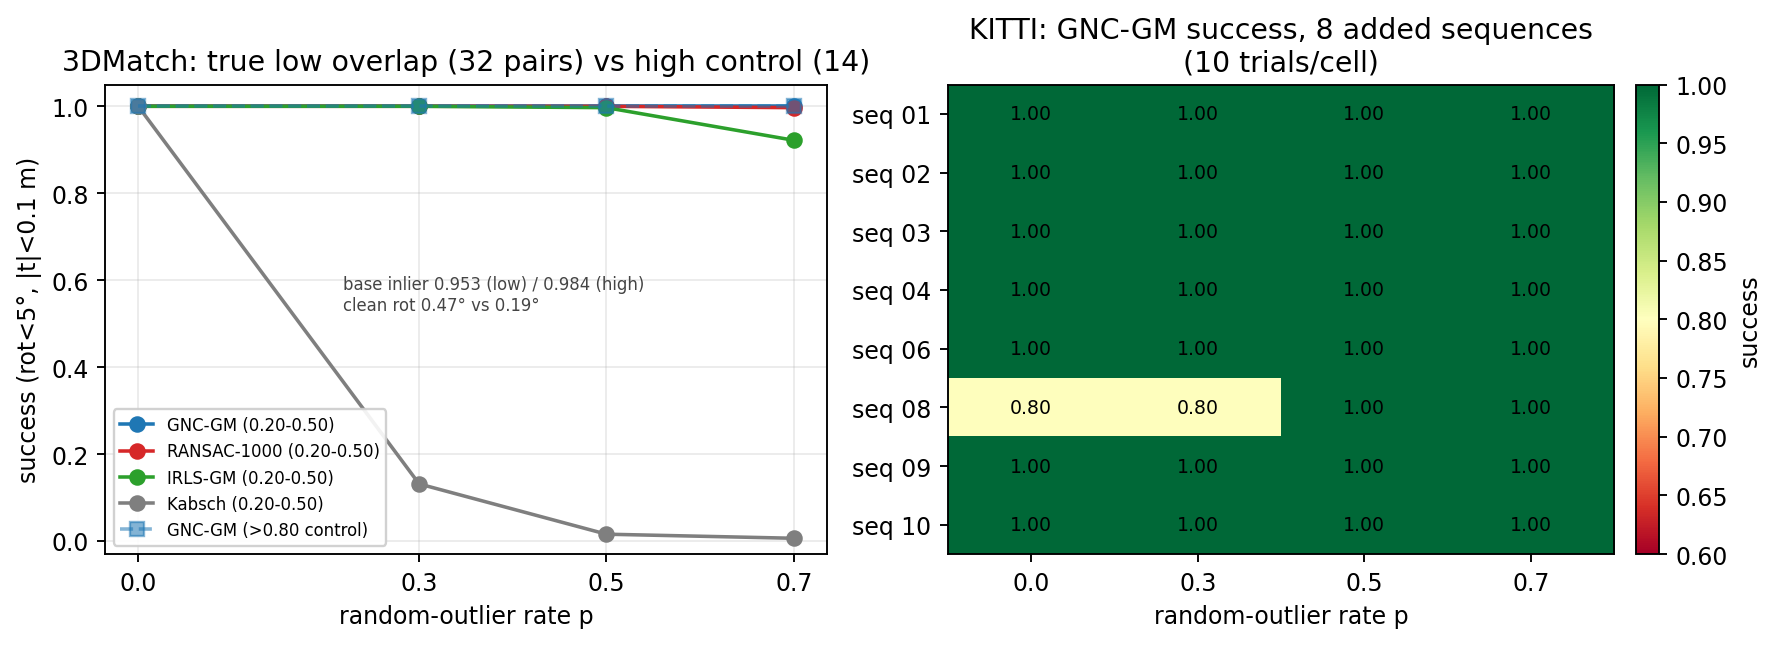
\includegraphics[width=0.75\columnwidth]{p3_data_coverage.png}
\caption{真实数据覆盖。左：3DMatch低重叠（$0.20$--$0.50$，32对）相对高重叠对照（14对），
每格10次试验。右：GNC-GM在新增八个KITTI odometry序列上的成功率；seq~08在$p=0$和$p=0.3$时
为$80\%$。}
\label{fig:coverage}
\end{figure}

\subsection{系统、基线与消融}

一个在$(B,N,3)$上向量化的NumPy GNC把循环复现到$1.1\times10^{-14}$（旋转）与
$1.2\times10^{-15}$（平移）；$B=32,N=100$时批处理p50为$8.5$~ms vs $56.2$~ms（$6.60\times$），
$B=8$给出$2.95\times$/$3.27\times$，$B=1$更慢（$0.54\times$）。$4\times4$的Davenport/Horn
内层求解器\cite{horn1987}在数值上等价于加权Kabsch（最大$\|R_d-R_k\|_F=1.07\times10^{-14}$，
代价超出$9.4\times10^{-16}$），但只在大$N$时更快。在合成数据上，Theseus-GM随机初始化下
$p=0/0.3/0.5/0.7$时为$100/80/55/25\%$，耗时$358$--$670$~ms，而GNC-GM在同一20个实例上以
$1.7$~ms达到$100\%$（$p=0.3$的Wilson区间重叠）；SDPRLayers+SCS数值上可用（$0/208$异常，
$8.5$--$13.4$~ms），但只在$p=0$成功，且$W_i=I$时退化为Kabsch。核、调度、RANSAC强度与
各向异性权重消融见附录~\ref{app:ablations}。

\section{讨论与局限}
\label{sec:discussion}

\noindent\textbf{局限与未来工作。}该层微分的是一个局部鲁棒不动点：外层GNC不是全局求解器，不
提供崩溃点保证，相干多数外点还可能使鲁棒全局最优本身出错。外部基线（Theseus-GM与
SDPRLayers+SCS）仅在合成3D--3D上评测，真实数据前端为手写的（SIFT+StereoSGBM与FPFH），夜间
In-The-Dark证据为10对窗口，且未使用学习描述子。将评测扩展到学习前端、真实数据外部基线与整夜
序列是自然的下一步；通用40根QPEP内层求解器与GPU批处理留作未来工作。

\noindent\textbf{模型崩溃。}即使$F_{\mathrm{rob}}$有完美的全局求解器，当相干外点多于内点时它
也可能返回错误位姿。一个一维例子：一个内点在$0$、两个相干外点在$M$，当$M\to\infty$时
$F(0)\to2c^2$、$F(M)\to c^2$，故全局极小是外点位姿。这一可辨识性极限需要一致性检查、内点计数
诊断或外点比例先验。

\noindent\textbf{边界残差。}$\lambda_\parallel$在$e=c^2$处最负，而不是在$e\to\infty$处。粗大
外点在$O(\|\mathbf{r}\|^{-4})$意义下被抑制，但刚好越过重降阈值的点具有最大的梯度影响，故边界
残差既是训练中最敏感的部分，也是曲率修正最关键之处。

\noindent\textbf{相对RANSAC的运行时间。}RANSAC是强且调优良好的基线，该层去掉其不可微外壳的
代价是局部鲁棒估计器。相对固定预算RANSAC，加速为$22$--$32\times$；相对自适应预算RANSAC，在
低外点比例更慢，$40\%$附近持平，$70\%$时约快$8\times$；LO-RANSAC精度持平，但比自适应RANSAC
慢$1.03$--$1.52\times$，因此比较必须注明迭代预算。

\noindent\textbf{核尺度与残差模型。}框架覆盖GM、Cauchy、Welsch与TLS，但尺度$c$至关重要：
固定$c$可能在变化噪声下失效，学习的$c$需要$\det W_i=1$之类归一化。这些推导对关于$\mathbf{t}$
仿射、关于提升四元数二次的残差是精确的；重投影误差不是多项式，QPEP在该情形使用代数代理。

\noindent\textbf{适用范围。}当匹配含粗大外点、需要穿过位姿的端到端梯度、外点比例低于崩溃区，
且$6\times6$反向与固定规模代数前向符合预算时，该层适用；当目标是全局最优性时，可认证全局求解器
仍是更合适的选择。

\section{结论}
\label{sec:conclusion}

我们提出了Robust-QPEPLayer，一种无RANSAC的可微位姿层，融合BR对偶、GNC与恒定规模的QPEP内层
求解器，并精确微分鲁棒不动点。理论隔离出自然实现会丢掉的两项：重降曲率修正（即BR权重块的
Schur补）与单位四元数约束乘子。一维符号翻转命题给出了冻结权重梯度符号错误的严格设定，逐观测
$O(\|\mathbf{r}\|^{-4})$界量化了粗大外点的梯度衰减。精确IFT Jacobian与中心有限差分吻合到
$3$--$5\times10^{-8}$，而冻结权重在边界处的相对误差为$1.07$、余弦为$0.234$。在合成数据、
ModelNet40/10、八个3DMatch场景、两次KITTI驾驶、11个KITTI odometry序列00--10以及四次
In-The-Dark运行上，GNC-GM在$70\%$随机外点以内与固定1000次RANSAC成功率相当，运行时间低
$22$--$32\times$；In-The-Dark误差为$0.078$--$0.150^\circ$与$0.007$--$0.020$~m。


% 参考文献：条目见 refs.bib（与英文源树一致，未增删）。
% 采用 unsrt 样式：编号按正文首次引用顺序，与英文稿的 IEEEtran 编号习惯一致。
\bibliographystyle{unsrt}
\bibliography{refs}


% ---------------------------------------------------------------- appendix
% 不计入七页正文限制。\newpage 使边界显式，附录起始页码即正文页数
% （用 \pageref{app:start} 核对）。
\newpage
\section*{附录：详细结果（不计入正文页数限制）}
\label{app:start}

本附录\emph{不}计入正文页数限制。它汇集证据状态表、证明与算法细节、核对偶表、支撑
表~\ref{tab:real}的逐数据集与逐场景数字、系统/基线/消融细节，以及反证。除明确标注外，每条记录
均为来自\texttt{experiments/}的独立复现。

\begin{figure}[t]
\centering
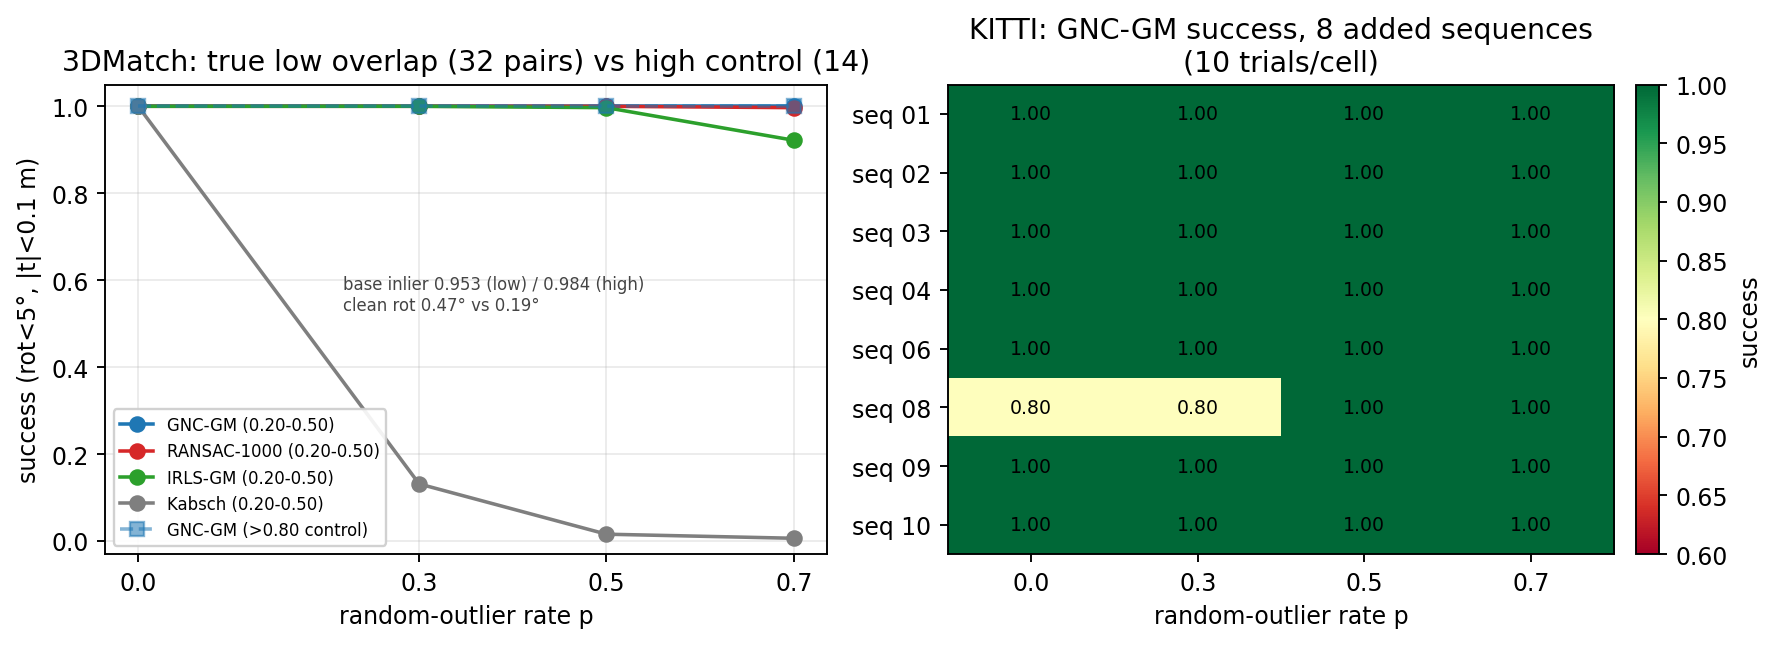
\includegraphics[width=\columnwidth]{p3_data_coverage.png}
\caption{超出原计划的数据覆盖。左：3DMatch真实低重叠带（$0.20$--$0.50$几何重叠，32个低重叠对）
与高重叠对照（14对），每格10次试验；oracle基础内点$0.953$（低） vs $0.984$（高），干净旋转
$0.47^\circ$ vs $0.19^\circ$；GNC-GM与RANSAC-1000保持$100\%$，IRLS在$p=0.7$达到$92\%$，
Kabsch崩溃到$1\%$。右：GNC-GM在新增八个KITTI odometry序列上的成功率（每格10次试验）；
seq~08是唯一真实的坏盆失效（$p=0$和$p=0.3$时为$80\%$）。来源：
\texttt{experiments/real/p3\_data\_coverage.png}。}
\label{fig:coverage}
\end{figure}

\subsection*{A. 证明、推导注记与反向算法}
\label{app:proofs}
\label{app:backward}

引理~\ref{lem:brdual}--\ref{lem:weights}、定理~\ref{thm:gnc}--\ref{thm:rhs}、
命题~\ref{prop:signflip}--\ref{prop:bound}的完整证明，Schur补恒等式、黎曼Hessian公式与存在性
构造，均维护在项目理论笔记（\texttt{theory/proofs.md}与\texttt{theory/derivations.md}）中；
数值检查在\texttt{verify/}中。正文给出适合页数预算的结果与证明梗概。具体而言：

\begin{itemize}
\item \emph{引理~\ref{lem:brdual}}：$w\mapsto we+\psi_\mu(w)$在$(0,1]$上严格凸、驻点为
  $w^*$；代入$w^*$即恢复$\rho_\mu(e)$，且盒约束是笛卡尔积，故多观测极小问题可分离。
\item \emph{引理~\ref{lem:schur}}：对联合目标在$(z,w)$上求微分得到$H_J$；利用
  $\psi''(w_i^*)=-1/\rho''(e_i^*)>0$消去$\delta w$，得到
  $H_{\mathrm{rob}}=H_{\mathrm{IRLS}}+\Delta H_{\mathrm{redesc}}$。
\item \emph{引理~\ref{lem:hessian}}：对$f\in C^2(\mathcal{M})$，限制在切空间上的欧氏Hessian与
  黎曼Hessian相差第二基本形式，对单位球面它贡献
  $-(\mathbf{q}^\top G_q)\diag(I_4,0_3)$ \cite{absil2008}。对3D--3D，
  $g_{i,q}^E=2J_i^\top W_i\mathbf{r}_i$且$J_i\mathbf{q}=2\mathbf{u}_i$，故
  $\lambda_i=\mathbf{q}^\top g_{i,q}^E=4\mathbf{u}_i^\top W_i\mathbf{r}_i$。$W_i(\theta)$扩展
  在$\partial e_i/\partial\theta$中增加
  $2\mathbf{r}_i^\top(\partial W_i/\partial\theta)\mathbf{r}_i$，并保持固定$W_i$处的Hessian
  不变。
\item \emph{命题~\ref{prop:existence}}：在$t=0$与$t=Kc^4/d^3$（$d=y_2-y_1$）处计算
  $\Phi(t)=\sum_i2\rho'(e_i)(t-y_i)$的符号，并利用$d\to\infty$时
  $H_{\mathrm{rob}}\to\lambda_\parallel(0)=2>0$。
\item \emph{命题~\ref{prop:bound}}：常数由
  $\|\partial\Phi/\partial\mathbf{y}_i\|_F\le Cc^4/(c^2+e_i)^2$、
  $\lambda_{\min}(H_{\mathrm{rob}})\ge\mu_0$、$W_i=I$时$\|\mathbf{r}_i\|^2=e_i$，以及
  $\|\rho'(e_i)g_i\|\le2\overline wc^4/\|\mathbf{r}_i\|^3$推出。
\end{itemize}

\begin{algorithm}[t]
\caption{精确反向传播（鲁棒不动点的隐式微分）}
\label{alg:backward}
\footnotesize
\begin{algorithmic}[1]
\Require 上游梯度；缓存的$z^*,w^*,e^*$
\For{$i=1$ to $N$}
  \State 计算$\mathbf{u}_i,\mathbf{r}_i,J_i,g_i^E\in\mathbb{R}^7,H_i^E\in\mathbb{R}^{7\times7}$
\EndFor
\State $G\gets\sum_i\rho'_i g_i^E$；\quad
       $H_E\gets\sum_i\big(\rho'_iH_i^E+\rho''_ig_i^Eg_i^{E,\top}\big)$
\State $B_q\gets$ $\mathbf{q}^{*\perp}$的正交基；\quad $B\gets\diag(B_q,I_3)$
\State $H_{\mathrm{rob}}\gets B^\top H_EB-\lambda_{\mathrm{rob}}\diag(I_3,0_3)$，\quad
       $\lambda_{\mathrm{rob}}=\mathbf{q}^{*\top}G_q$
\State $\mathrm{RHS}\gets\sum_i\rho'_i\,\mathrm{d}g_i/\mathrm{d}\theta
       +\sum_i\rho''_ig_i(\mathrm{d}e_i/\mathrm{d}\theta)^\top$
\State $\mathrm{d}z\gets\mathrm{solve}(H_{\mathrm{rob}},-\mathrm{RHS})$
\State 将$\mathrm{d}z$链式回传至$(\mathbf{q},\mathbf{t})$及上游损失
\end{algorithmic}
\end{algorithm}

\begin{figure}[t]
\centering
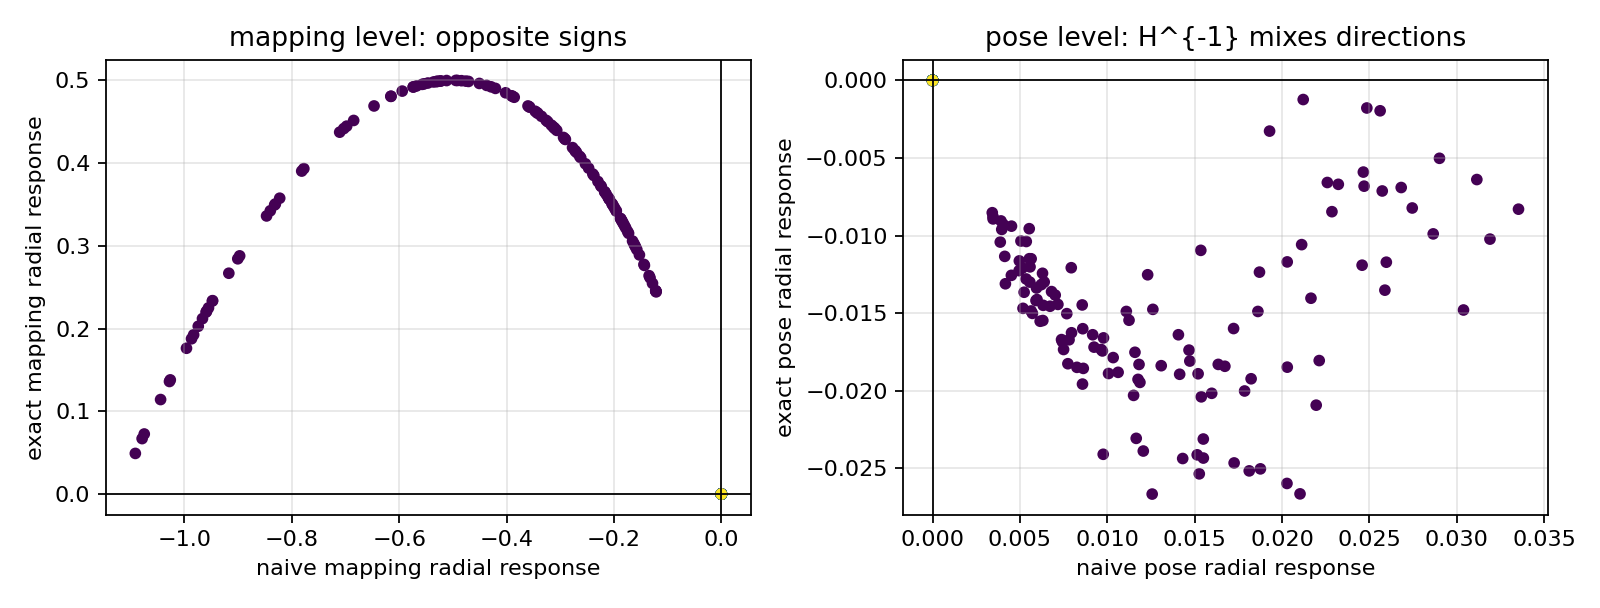
\includegraphics[width=\columnwidth]{gradient_sign.png}
\caption{命题~\ref{prop:signflip}背后的数值符号结构。左：映射级径向响应，精确 vs 冻结权重
（朴素）；当$e>c^2/3$时符号相反。右：经$H_{\mathrm{rob}}^{-1}$后的位姿级响应；逆Hessian混合
各方向，故6D符号是数值观察而非定理。来源：
\texttt{synthetic/results/gradient\_sign.png}。}
\label{fig:sign}
\end{figure}

\subsection*{B. 每条声称的证据状态}
\label{app:status}

表~\ref{tab:status}把理论、测量与受阻工程之间的边界显式化，使任何已度量行都不会被读作理论保证，
任何未来行都不会被读作结果。

\begin{table*}[t]
\caption{本文声称的证据状态（v0.4一致性检查）。产物位于
\texttt{labs/03-robust-qpeplayer/}下。}
\label{tab:status}
\centering
\scriptsize
\setlength{\tabcolsep}{3pt}
\begin{tabular}{@{}>{\raggedright\arraybackslash}p{4.2cm}
  >{\raggedright\arraybackslash}p{2.6cm}
  >{\raggedright\arraybackslash}p{6.6cm}
  >{\raggedright\arraybackslash}p{1.4cm}@{}}
\toprule
条目 & 状态 & 证据 & 章节 \\
\midrule
BR对偶、GNC不动点驻性、Schur补曲率修正、精确黎曼Hessian、一维符号翻转、存在性、
$O(\|\mathbf{r}_i\|^{-4})$界 & 新理论（证明+数值检查） & \texttt{theory/proofs.md}、
\texttt{verify/}、\texttt{synthetic/results/verify\_smoke.txt} & \S\ref{sec:method} \\
精确IFT反向 vs 中心FD（600个观测，6D） & 已度量 &
\texttt{synthetic/results/gradient\_table.json} & \S\ref{sec:experiments} \\
GNC-GM vs 固定/自适应RANSAC（随机、相干、边界外点） & 已度量（合成、ModelNet40/10、全部8个
官方3DMatch测试场景、2次KITTI raw驾驶、全部11个odometry序列） &
\texttt{synthetic/results/main\_table\_extended.json}、\texttt{real/*/results/*.json} &
\S\ref{sec:experiments} \\
端到端边界精化，NumPy与torch & 已度量的玩具诊断（GT监督，5--10个种子；非学习系统） &
\texttt{synthetic/results/e2e\_table.json}、\texttt{e2e\_torch/results/*.json} &
\S\ref{sec:experiments} \\
Theseus-GM与SDPRLayers+SCS & 仅在合成3D--3D上度量（SDPR为前向，$W_i=I$时退化为Kabsch） &
\texttt{baselines/results/baselines.json} & \S\ref{sec:experiments} \\
UTIAS In-The-Dark & 在两次白天+两次夜间前缀运行上的度量协议（复合官方GT、手写SIFT+SGBM）；
整夜/训练前端未测试 & \texttt{real/inthedark/results/} & \S\ref{sec:experiments} \\
KITTI双目回退 & 已度量的负结果（旋转可解，平移受前端限制） &
\texttt{real/kitti\_stereo/results/} & \S\ref{sec:experiments} \\
6D符号翻转陈述 & 不是定理；仅为数值观察 & \texttt{gradient\_table.json} &
\S\ref{sec:signflip} \\
通用40根QPEP多项式求解器 & 未实现（所有表格使用标量权重$4\times4$特化） &
\texttt{qpep\_gpu/qpep\_scope.md} & \S\ref{sec:experiments} \\
$4\times4$内层的GPU计时/CUDA-graph捕获 & 因Slurm GPU占用受阻；仅CPU验证 &
\texttt{qpep\_gpu/results/qpep\_gpu.json}、\texttt{logs/slurm\_gpu\_*} &
\S{}E \\
学习描述子（FCGF/Predator）、真实数据外部基线、端到端训练的In-The-Dark、完整54场景3DMatch
训练语料 & 未来工作 & --- & \S\ref{sec:notmeasured} \\
\bottomrule
\end{tabular}
\end{table*}

\subsection*{C. 核对偶}
\label{app:kernel}

表~\ref{tab:kernel}列出该层使用的BR对偶，其中$a=\mu c^2$。前向与反向在不同核之间结构完全相同：
只有$\rho_\mu'$与$\psi_\mu''$改变。TLS具有线性的$\psi$，且在$e=a$处权重不唯一；它需要GNC-TLS
调度，而不是单纯的带宽退火。

\begin{table}[t]
\caption{四种核的Black--Rangarajan对偶（$a=\mu c^2$）。来源：
\texttt{theory/derivations.md}，由\texttt{verify/}复现。}
\label{tab:kernel}
\centering
\scriptsize
\setlength{\tabcolsep}{1.5pt}
\begin{tabular}{llll}
\toprule
核 & $\rho_\mu(e)$ & $w^*=\rho_\mu'(e)$ & $\psi_\mu(w)$ \\
\midrule
Geman--McClure & $ae/(a+e)$ & $(a/(a+e))^2$ & $a(\sqrt{w}-1)^2$ \\
Cauchy & $a\log(1+e/a)$ & $a/(a+e)$ & $a(w-1-\log w)$ \\
Welsch & $a(1-e^{-e/a})$ & $e^{-e/a}$ & $a(1-w+w\log w)$ \\
TLS & $\min(e,a)$ & \shortstack[l]{$1$ (若$e<a$)\\$0$ (若$e>a$)} & $a(1-w)$ \\
\bottomrule
\end{tabular}
\end{table}

\subsection*{D. 逐数据集结果}
\label{app:datasets}

\noindent\textbf{ModelNet40/10。}表~\ref{tab:modelnet}给出汇总数字。ModelNet10使用10类共908个
测试物体，OFF网格重采样到2048点；鲁棒方法的成功率与ModelNet40最多相差$2$个百分点，中位旋转最多
相差$0.038^\circ$。

\begin{table*}[t]
\caption{均匀随机外点下的ModelNet物体点云结果，每格50次试验，$N=100$，$c=0.05$~m。来源：
\texttt{real/modelnet/results/main\_table.json}、
\texttt{real/modelnet10/results/main\_table.json}。}
\label{tab:modelnet}
\centering
\scriptsize
\setlength{\tabcolsep}{3pt}
\begin{tabular}{lcccccc}
\toprule
数据集 & GNC & RANSAC-1000 & IRLS & Kabsch & GNC ms & RANSAC ms \\
\midrule
ModelNet40 & $100\%$ $\le70\%$ & $100\%$ & $98$--$100\%$ & 崩溃$\ge50\%$ & $1.7$--$1.9$ & $53.5$--$61.5$ \\
ModelNet10 & $100\%$ $\le70\%$ & $100\%$ & $98$--$100\%$ & 崩溃$\ge50\%$ & $1.7$--$1.9$ & $53.5$--$61.5$ \\
\bottomrule
\end{tabular}
\end{table*}

\noindent\textbf{3DMatch。}表~\ref{tab:3dmatch}给出八场景汇总行、低/中/高重叠研究、更严格的
$0.20$--$0.50$带，以及两次FPFH前端审计。对全部八个官方测试场景汇总（每格20次试验），$p=0.7$
时GNC p50为$2.26$~ms，而固定1000 RANSAC为$62.6$~ms（$27.7\times$），$p=0.7$时边界中位旋转为
$0.27^\circ$ vs $0.52^\circ$。逐场景GNC p50为$2.26$--$2.36$~ms vs $62.1$--$73.4$~ms
（$27.4$--$31.1\times$），IRLS在$70\%$时为$99\%$，相干外点在$60$--$70\%$时所有方法均崩溃
（$0\%$）。重叠研究为高/中/低分箱选择24/21/20对；干净旋转为$0.18^\circ$/$0.24^\circ$/
$0.52^\circ$，但GNC与RANSAC在每个分箱、$p=0.7$时均保持$100\%$，成功差为零，$p\ge30\%$时加速
$27.7$--$30.4\times$。低分箱的中位基础内点比例仍为$0.95$。更严格的$0.20$--$0.50$几何重叠带
（每场景4个低重叠+2个匹配高重叠对，每格10次试验）的oracle基础内点为$0.953$（低）/$0.984$
（高），干净旋转$0.47^\circ$/$0.19^\circ$；GNC与RANSAC-1000在$p=0.7$时为$100\%$，IRLS为
$92\%$，Kabsch为$1\%$。低重叠减少的是可用对应的\emph{数量}，而非oracle内点比例。FPFH前端
（互为最近邻加成对距离一致性，匹配中不使用GT）在两个被审计场景上达到$80.0\%$与$67.8\%$的
自然内点率。

\begin{table*}[t]
\caption{3DMatch细节。oracle对应使用真实重叠片段上的GT映射最近邻；FPFH行使用手工前端且匹配中
不含GT（不是FCGF/Predator）。“bnd”$=$边界外点。来源：
\texttt{real/threedmatch\_full/results/full\_scenes.json}、
\texttt{overlap\_bins.json}、\texttt{overlap\_dependence.json}；
\texttt{real/threedmatch/results/descriptor.json}。}
\label{tab:3dmatch}
\centering
\scriptsize
\setlength{\tabcolsep}{3pt}
\begin{tabular}{lcccccc}
\toprule
设置 & 对数/试验数 & 干净旋转 & GNC & RANSAC-1000 & Kabsch & 加速 \\
\midrule
汇总8个测试场景，随机 & 每场景8对，每格20次 & --- & $100\%$ $\le70\%$ & $100\%$ & --- & $27.7\times$ @$70\%$ \\
汇总8个测试场景，bnd.@$70\%$ & 每场景8对，每格20次 & --- & $0.27^\circ$ & $0.52^\circ$ & --- & --- \\
重叠高 & 24对 & $0.18^\circ$ & $100\%$ @$0.7$ & $100\%$ & --- & $27.7$--$30.4\times$ \\
重叠中 & 21对 & $0.24^\circ$ & $100\%$ @$0.7$ & $100\%$ & --- & $27.7$--$30.4\times$ \\
重叠低 & 20对 & $0.52^\circ$ & $100\%$ @$0.7$ & $100\%$ & --- & $27.7$--$30.4\times$ \\
严格$0.20$--$0.50$带 & 每场景4低+2高对，每格10次 & $0.47^\circ$ / $0.19^\circ$ & $100\%$ @$0.7$ & $100\%$ & $1\%$ & --- \\
FPFH审计1 & 自然内点$80.0\%$ & --- & $100\%$ & $100\%$ & $100\%$ & --- \\
FPFH审计2 & 自然内点$67.8\%$ & --- & $100\%$ & $97\%$ & $83\%$ & --- \\
\bottomrule
\end{tabular}
\end{table*}

\noindent\textbf{KITTI。}表~\ref{tab:kitti}汇集raw驾驶与odometry行。对raw驾驶，自运动来自OXTS
（Mercator加横滚/俯仰/偏航），并用\texttt{calib\_imu\_to\_velo}映射到Velodyne；方向已验证
（drive 0001正确NN $0.100$--$0.123$~m vs 逆$0.143$--$0.183$~m；drive 0002 $0.108$--$0.140$~m
vs $0.136$--$0.269$~m）。Drive 0002精确复现drive-0001的随机与边界表格，保持相干转变
（$50\%$时GNC $40\%$ vs $35\%$，IRLS $30\%$ vs $45\%$；二者均为随机水平），并给出
$\sim21$--$23\times$的加速。阈值扫描使GNC在$c\in\{0.15,0.25,0.35\}$时保持$100\%$，其中
$c=0.25$是与$\sim0.10$~m点间距最合理的匹配。对odometry，仅从84.8~GB官方归档中按范围抓取每序列
32--33个触及帧，故全部11个序列00--10都有代表。在新增八个序列上（每格10次试验），$p=0.7$时GNC
与RANSAC-1000均为$100\%$，唯seq~08例外（$p=0$和$p=0.3$时$80\%$，真实的坏盆失效；RANSAC为
$100\%$）；11个序列汇总的成功率为$p=0/0.3/0.5/0.7$时$99/99/100/100\%$，$p\ge0.3$时固定
RANSAC/GNC运行时间比为$22.4\times$。00/05/07子集给出失效模式细节：全部18次方向检查通过
（前向NN $0.053$--$0.114$~m vs 逆$0.104$--$0.430$~m），随机成功率在$70\%$以内为$100\%$，
汇总GNC $2.8$~ms vs $73.7$~ms（$26.3\times$），$p=0.6$时相干崩溃（$p=0.5$时GNC $53\%$，
IRLS $38\%$，RANSAC $0\%$），边界$0.067^\circ$ vs $0.143^\circ$，且在
$|\mathbf{t}|=0.09$--$9.62$~m与间隔$1/2/4/8$（171个配对单元格）上GNC从未低于RANSAC。精确位姿
的干净下限（$0.042$--$0.057^\circ$）并不低于OXTS raw驾驶（$0.030$--$0.039^\circ$），故主导它
的是LiDAR采样/体素化。每序列33帧是子集，不是完整流。

\begin{table*}[t]
\caption{KITTI raw驾驶与odometry，$N=300$，$c=0.25$~m，每格20次试验（新增序列每格10次）。除
seq~08外，随机外点成功率在$70\%$以内GNC与固定1000 RANSAC均为$100\%$。来源：
\texttt{real/kitti/results/kitti.json}、\texttt{real/kitti2/results/kitti2.json}、
\texttt{real/kitti\_odom/results/kitti\_odom.json}。}
\label{tab:kitti}
\centering
\footnotesize
\setlength{\tabcolsep}{4pt}
\begin{tabular}{lcccccc}
\toprule
序列 & 帧/对 & GNC p50 & RANSAC p50 & 加速 & 相干@$50\%$ & bnd.\ 旋转 \\
\midrule
raw 0001 & 108帧，10对 & $2.7$--$2.8$~ms & $61$--$64$~ms & $\sim22\times$ & 全部$0\%$ & $0.07$--$0.09^\circ$ \\
raw 0002 & 77帧，10对 & $2.7$--$2.8$~ms & $61$--$64$~ms & $\sim21$--$23\times$ & $40/35/30/45\%$ & $0.07$--$0.09^\circ$ \\
odom 00--10 & 每个33帧，汇总 & $2.8$~ms & $73.7$~ms & $22.4\times$ & seq~08 $80\%$ @$p\le0.3$ & --- \\
odom 00/05/07 & 每个33帧 & $2.8$~ms & $73.7$~ms & $26.3\times$ & $53/38/0\%$ & $0.067/0.143^\circ$ \\
\bottomrule
\end{tabular}
\end{table*}

\noindent\textbf{In-The-Dark。}表~\ref{tab:inthedark}给出白天运行与夜间窗口。复合官方GT已在不相交
对上用双目重投影验证：前向中位$0.65$~px（run\_000002）与$0.52$~px（run\_000012），而逆为
$18.1/27.9$~px、恒等为$9.5/14.7$~px、未共轭为$21.5/31.3$~px。所有检查通过（$512\times384$
图像，左右行对齐$0.56$--$0.58$~px）。归档为905~MB，但只按范围抓取315{,}463字节的变换文件
（CRC已验证）。夜间zip（2.6--2.76~GB）未下载；只抓取了触及的窗口。运动匹配的白天对照
（run\_000002起点757，$|\mathbf{t}|=0.21$~m，旋转$0.54^\circ$）给出$85.9\%$内点与
$0.121^\circ/0.007$~m；夜间中位深度为$4.5$~m，白天为$6.7$--$7.2$~m，故夜间内点率是几何效应，
不是SIFT在黑暗中更鲁棒的证据。

\begin{table*}[t]
\caption{UTIAS In-The-Dark：两次白天运行（各15对连续图像）与两个夜间前缀窗口（各10对）；手写
SIFT+StereoSGBM前端，无训练。GT重投影列为中位像素（前向 / 逆 / 恒等 / 未共轭车辆系）。来源：
\texttt{real/inthedark/results/inthedark\_dense.json}、
\texttt{inthedark\_run12\_dense.json}、\texttt{inthedark\_night.json}、
\texttt{verify\_run\_000002.json}、\texttt{verify\_run\_000012.json}。}
\label{tab:inthedark}
\centering
\scriptsize
\setlength{\tabcolsep}{2.2pt}
\begin{tabular}{llcccccc}
\toprule
运行 & 对数 & 内点率 & 旋转 & 平移 & 成功@$0.1$~m & Kabsch & GT重投影 \\
\midrule
白天 run\_000002 & 15 & $79.4\%$ & $0.078^\circ$ & $0.020$~m & $100\%$ & $47\%$ & $0.65/18.1/9.5/21.5$ \\
白天 run\_000012 & 15 & $88.5\%$ & $0.092^\circ$ & $0.010$~m & $100\%$ & $40\%$ & $0.52/27.9/14.7/31.3$ \\
夜间 run\_000017 & 10 & $96.0\%$ & $0.135^\circ$ & $0.011$~m & $100\%$ & --- & --- \\
夜间 run\_000018 & 10 & $97.1\%$ & $0.150^\circ$ & $0.011$~m & $100\%$ & --- & --- \\
夜间稀疏 & 10 & $84.3\%$ & $0.197^\circ$ & $0.015$~m & --- & --- & --- \\
白天对照 & 10 & $85.9\%$ & $0.121^\circ$ & $0.007$~m & --- & --- & --- \\
\bottomrule
\end{tabular}
\end{table*}

\noindent\textbf{KITTI双目回退（平移为负）。}drive 0001的三十对帧，在矫正后的
\texttt{image\_02/03}（$b=0.5327$~m）上使用SIFT+亚像素+StereoSGBM，给出$17.8\%$的自然内点率
（$c=0.5$~m），每对890个对应。GNC/IRLS把旋转恢复到$0.052^\circ$，而GT内点下限为$0.071^\circ$；
但平移中位$0.70$~m vs $1.92$~m运动与$0.239$~m下限；没有方法达到$0.1$~m或$0.25$~m成功。GNC
比固定1000 RANSAC快$19.3\times$（4.21 vs 81.3~ms）。$3$--$60$~m上双目与LiDAR深度比为
$1.000$--$1.061$，排除视差尺度缺陷；残差是来自前端、遮挡与动态偏置的相干前向平移低估
（$0.63$--$0.73$）。

\subsection*{E. 系统、批处理与内层求解器}
\label{app:systems}

一个在$(B,N,3)$上向量化的numpy GNC以相同的$\mu$-调度把循环复现到旋转
$\le1.1\times10^{-14}$、平移$\le1.2\times10^{-15}$。$B=32,N=100$时批处理p50为$8.5$~ms，而
循环为$56.2$~ms（$6.60\times$）；$B=8$时加速为$2.95\times$（$N=100$）与$3.27\times$
（$N=500$）；$B=1$更慢（$0.54\times$），故对单实例循环仍是正确选择。在RTX 5090的float64
eager torch上，GPU受启动开销限制于$42.4$--$45.7$~ms：在$B\le8$时落后
（$0.04$--$0.57\times$），$B=32,N=100$时大致持平（$1.33\times$），在$B=32,N=500$
（$2.23\times$）与$B=128$（$N=100$时$4.96\times$，$N=500$时$8.24\times$）时胜出。后续探针把
这一测试扩展到静态形状$4\times4$特征求解器与CUDA-graph捕获，覆盖
$B\in\{1,8,32,128,512\}$、$N\in\{100,500\}$、float64与float32。其CPU验证发现并修复了手写
Jacobi特征求解器中的一个Givens符号缺陷（修复前：static-jacobi与NumPy最大差
$\|\Delta R\|_F\approx1.80$，且只匹配$50\%$的$\mu$-调度；修复后：$\sim10^{-16}$且$100\%$
匹配）。

\textbf{GPU支路未被度量。}2026-11-28T00:26:08，我们向\texttt{gpu}分区提交作业3184
（\texttt{probe.py}、\texttt{--gres=gpu:1}、20~min）；00:31:16时
\texttt{scontrol show job 3184}报告\texttt{JobState=PENDING}、\texttt{Reason=Resources}、
\texttt{StartTime=2026-11-28T21:23:07}（约21~h之后），而作业3151/3180/3181占着三块RTX 5090。
该作业于00:31:21被取消，随后\texttt{scontrol}报告\texttt{JobState=CANCELLED}、
\texttt{Reason=Resources}；\texttt{squeue}/\texttt{scontrol}输出在
\texttt{experiments/qpep\_gpu/\allowbreak results/logs/\allowbreak slurm\_gpu\_3184\_state.txt}中。由于没有捕获任何
计算图，我们不声称任何CUDA-graph错误，也不涉及40根QPEP求解器。

$4\times4$的Davenport/Horn内层求解器 \cite{horn1987}在数值上等价于加权Kabsch（最大
$\|R_d-R_k\|_F=1.07\times10^{-14}$，最大代价超出$9.4\times10^{-16}$），但其运行时间只在大$N$
时更优：p50比为$0.94\times$（$N=20$）、$1.02\times$（$N=100$）、$1.28\times$（$N=500$），
几何平均$1.07\times$。它是大$N$选项，不是$N=100$的默认胜出项。

\begin{figure}[t]
\centering
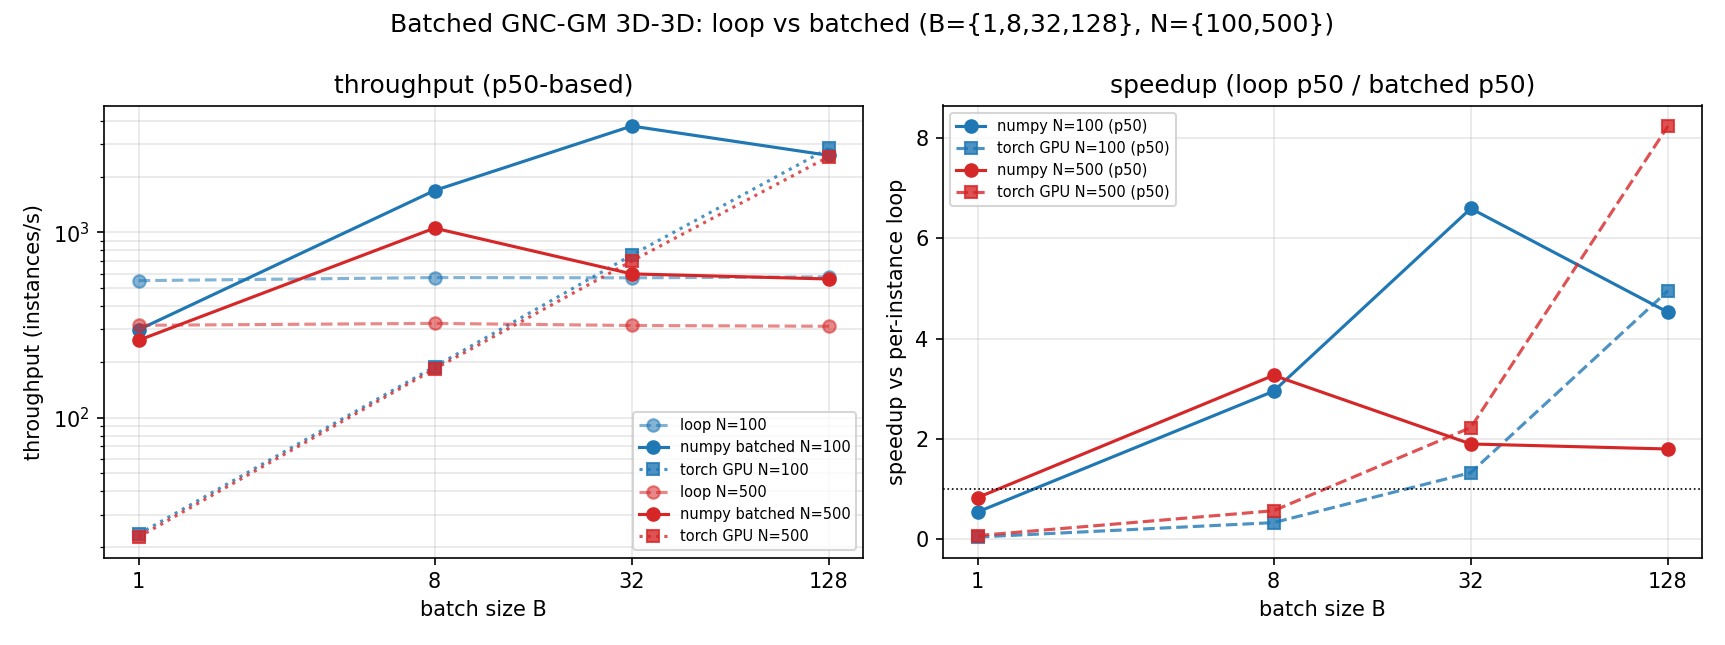
\includegraphics[width=\columnwidth]{batch_gnc.png}
\caption{$(B,N,3)$上的批处理GNC-GM：$B=\{1,8,32,128\}$与$N=\{100,500\}$的吞吐量与
循环对批处理的加速。GPU点为RTX 5090 float64 eager-torch批处理基准；它们不是受阻的静态形状
$4\times4$/CUDA-graph探针。来源：\texttt{systems/results/batch\_gnc.json}。}
\label{fig:batch}
\end{figure}

\subsection*{F. 外部基线（仅合成）}
\label{app:baselines}

Theseus 0.2.3（稠密Cholesky；无SuiteSparse头文件时\texttt{scikit-sparse}不可用）求解相同的逐点
GM目标；其Jacobian与有限差分的相对误差为$1.09\times10^{-10}$，GM代价精确一致。GT初始化下
Theseus-GM在所有$p$均$100\%$成功（局部盆检查，不是全局恢复）；随机初始化下在
$p=0/0.3/0.5/0.7$时成功率为$100/80/55/25\%$，p50为$358$--$670$~ms。在同一20个实例上，
GNC-GM在每个$p$均$100\%$，耗时$1.7$~ms，RANSAC-自适应为$100\%$、$0.2$--$14.1$~ms，而Kabsch
在$p\ge0.3$时失败。Theseus随机初始化在$p=0.3$的20次试验Wilson区间（$[0.58,0.92]$）与GNC的
$20/20$（$[0.84,1.00]$）重叠，故该差距不显著；$p=0.5/0.7$则已分离（表~\ref{tab:baselines}）。

\begin{table}[t]
\caption{合成外部基线，每个$p$有20个实例；$p=0/0.3/0.5/0.7$时的成功率（\%）与p50时间。来源：
\texttt{baselines/results/baselines.json}、\texttt{theseus.json}、
\texttt{sdpr\_forward.json}。}
\label{tab:baselines}
\centering
\scriptsize
\setlength{\tabcolsep}{1.8pt}
\begin{tabular}{lcccc}
\toprule
方法 & $p=0$ & $0.3$ & $0.5$ & $0.7$/时间 \\
\midrule
Theseus-GM，GT初值 & 100 & 100 & 100 & 100 \\
Theseus-GM，随机初值 & 100 & 80 & 55 & 25 / 358--670 \\
GNC-GM & 100 & 100 & 100 & 100 / 1.7~ms \\
RANSAC-自适应 & 100 & 100 & 100 & 100 / 0.2--14.1~ms \\
Kabsch & 100 & 失败 & 失败 & 失败 \\
SDPRLayers+SCS & 100 & 失败 & 失败 & 失败 / 8.5--13.4~ms \\
\bottomrule
\end{tabular}
\end{table}

SDPRLayers+SCS（cb3aed2处的新鲜\texttt{utiasASRL/sdprlayer}，SCS，208次前向）在数值上可用：
$0/208$次SCS异常，$8.5$--$13.4$~ms。它在$p=0$成功，但在$p\ge0.3$失败，这在无鲁棒核时符合
预期。$W_i=I$且权重为单位值时，其目标等于Kabsch：80次配对试验给出最大
$|\Delta R|=1.5\times10^{-5}$~度与最大$|\Delta t|=1.3\times10^{-9}$~m。该行是前向正确性/可用性
检查，\textbf{不是}独立的鲁棒基线；要得到有区别的SDPR，需要非单位的$W_i$（例如POLI）或
RANSAC。BPnP仅做3D--2D PnP，Pyatov等是两视图2D--2D，POLI是逐点几何估计器且未找到官方位姿
求解器代码/权重；它们都不是3D--3D基线，故没有编造任何表格。

\subsection*{G. 消融}
\label{app:ablations}

\noindent\textbf{核。}在相同的加权Kabsch内层与调度下，GM、Cauchy与Welsch在随机与边界外点上
$70\%$以内均为$100\%$（表~\ref{tab:kernelabl}）。GM在$50$--$70\%$时具有最低的边界中位旋转
（$0.199/0.229/0.340^\circ$ vs Cauchy $0.241/0.264/0.370^\circ$与Welsch
$0.220/0.268/0.392^\circ$）。没有证据支持更换默认核。

\begin{table}[t]
\caption{核消融：$p=0.5/0.6/0.7$时的边界中位旋转（度）；所有核在随机与边界外点上$70\%$以内
均为$100\%$。来源：\texttt{ablations/kernels/\allowbreak results/kernel\_ablation.json}。}
\label{tab:kernelabl}
\centering
\footnotesize
\setlength{\tabcolsep}{4pt}
\begin{tabular}{lccc}
\toprule
核 & $p=0.5$ & $p=0.6$ & $p=0.7$ \\
\midrule
GM（默认） & $0.199$ & $0.229$ & $0.340$ \\
Cauchy & $0.241$ & $0.264$ & $0.370$ \\
Welsch & $0.220$ & $0.268$ & $0.392$ \\
\bottomrule
\end{tabular}
\end{table}

\noindent\textbf{GNC调度。}扫描$\gamma\in\{1.2,1.4,1.7,2.0\}$、$\mu_0$乘子
$\{0.5,1,4\}$与精化步数$\{0,5,10\}$，在$p=0.3/0.5/0.7$时均给出$100\%$成功与相同的中位旋转；
$\gamma=2.0$比默认快$1.04$--$1.79\times$，$\gamma=1.2$慢$1.47$--$2.49\times$。默认是保守的，
不是唯一最优。

\noindent\textbf{RANSAC强度。}更强的LO-RANSAC（MSAC评分，最多五轮局部重拟合/重评分，0.999
自适应停止，上限1000）在精度上与GNC持平（中位旋转差$\le0.006^\circ$），但在每个$p$都比普通
自适应RANSAC慢$1.03$--$1.52\times$，因为最终一致性重拟合已经是同一个估计器。因此固定1000基线
在运行时间上是稻草人。

\noindent\textbf{各向异性$W_i$。}在Cholesky白化残差上使用正确的6-DoF Gauss--Newton内层求解时，
$W_i=I$与Kabsch吻合到$5.3\times10^{-13}$。标量加权Kabsch对各向异性$W_i$是\textbf{不}精确的：
在收敛的GM权重下其目标比为$1.002$--$1.007$（对角）与$1.035$--$1.088$（完整SPD），单次试验
最大为$3.80$。然而在各项同性合成噪声下，各向异性$W_i$是误设模型：完整$W$的GNC配对中位旋转
变化为$+0.055$到$+0.124^\circ$，仅在$8$--$32\%$的试验中更好，$p=0.7$时成功率为$92\%$
（单位权重：$100\%$）。精确内层求解比标量Kabsch慢$4.9$--$23\times$。故我们将其作为正确性/负
结果报告：当$W_i$确实各向异性时使用非线性内层，但不要声称在本数据上各向异性带来精度收益。

\subsection*{H. 反证}
\label{app:falsifiers}

可度量的声称都被写成可失败的形式：

\begin{itemize}
\item \textbf{精确反向。}若精确IFT Jacobian不再与精化分支上的中心有限差分吻合（相对Frobenius
  误差高于$10^{-6}$，或余弦低于$0.999$），则“精确不动点导数”的声称不成立。当前值为
  $4.9\times10^{-8}$/$3.1\times10^{-8}$（内点/边界），余弦$1.000000$。
\item \textbf{曲率修正。}若朴素冻结权重Jacobian不是边界观测上的主导误差源（例如无$\lambda$
  变体更差），则Schur补的解释无法说明测量。当前：边界上朴素$1.07$ vs 无$\lambda$
  $9.8\times10^{-4}$。
\item \textbf{符号翻转。}一维中命题即证明；数值上，若精确与朴素径向响应在$e>c^2/3$时没有
  相反符号，则6D诊断的数值前提失败。当前：$122/122$个边界与$64/64$个粗大观测翻转。
\item \textbf{前向鲁棒性。}若GNC-GM在随机外点上任一$p\in[0,0.7]$的成功率低于固定预算RANSAC，
  则“与固定预算RANSAC持平”的声称不成立。当前：在合成、ModelNet40/10、3DMatch、KITTI raw与
  odometry上持平。
\item \textbf{预算声称。}若自适应RANSAC在低$p$时比GNC慢，则所述“低$p$时更慢”的限定不成立。
  当前：GNC在$p=0.1$时慢$3.9\times$，在$p=0.7$时快$8.3\times$。
\item \textbf{可辨识性失效。}若任何方法在$60$--$70\%$相干外点下恢复了真值位姿，则模型崩溃的
  讨论有误。当前：所有方法都返回外点变换。
\item \textbf{真实数据范围。}若In-The-Dark GT在留出重投影上未能胜过逆/恒等/共轭替代，则“协议
  验证”的声称失败。当前：$0.52$--$0.65$~px vs $9.5$--$31.3$~px。
\end{itemize}


\end{document}
